% Options for packages loaded elsewhere
\PassOptionsToPackage{unicode}{hyperref}
\PassOptionsToPackage{hyphens}{url}
%
\documentclass[
]{article}
\usepackage{amsmath,amssymb}
\usepackage{iftex}
\ifPDFTeX
  \usepackage[T1]{fontenc}
  \usepackage[utf8]{inputenc}
  \usepackage{textcomp} % provide euro and other symbols
\else % if luatex or xetex
  \usepackage{unicode-math} % this also loads fontspec
  \defaultfontfeatures{Scale=MatchLowercase}
  \defaultfontfeatures[\rmfamily]{Ligatures=TeX,Scale=1}
\fi
\usepackage{lmodern}
\ifPDFTeX\else
  % xetex/luatex font selection
\fi
% Use upquote if available, for straight quotes in verbatim environments
\IfFileExists{upquote.sty}{\usepackage{upquote}}{}
\IfFileExists{microtype.sty}{% use microtype if available
  \usepackage[]{microtype}
  \UseMicrotypeSet[protrusion]{basicmath} % disable protrusion for tt fonts
}{}
\makeatletter
\@ifundefined{KOMAClassName}{% if non-KOMA class
  \IfFileExists{parskip.sty}{%
    \usepackage{parskip}
  }{% else
    \setlength{\parindent}{0pt}
    \setlength{\parskip}{6pt plus 2pt minus 1pt}}
}{% if KOMA class
  \KOMAoptions{parskip=half}}
\makeatother
\usepackage{xcolor}
\usepackage[margin=1in]{geometry}
\usepackage{color}
\usepackage{fancyvrb}
\newcommand{\VerbBar}{|}
\newcommand{\VERB}{\Verb[commandchars=\\\{\}]}
\DefineVerbatimEnvironment{Highlighting}{Verbatim}{commandchars=\\\{\}}
% Add ',fontsize=\small' for more characters per line
\usepackage{framed}
\definecolor{shadecolor}{RGB}{248,248,248}
\newenvironment{Shaded}{\begin{snugshade}}{\end{snugshade}}
\newcommand{\AlertTok}[1]{\textcolor[rgb]{0.94,0.16,0.16}{#1}}
\newcommand{\AnnotationTok}[1]{\textcolor[rgb]{0.56,0.35,0.01}{\textbf{\textit{#1}}}}
\newcommand{\AttributeTok}[1]{\textcolor[rgb]{0.13,0.29,0.53}{#1}}
\newcommand{\BaseNTok}[1]{\textcolor[rgb]{0.00,0.00,0.81}{#1}}
\newcommand{\BuiltInTok}[1]{#1}
\newcommand{\CharTok}[1]{\textcolor[rgb]{0.31,0.60,0.02}{#1}}
\newcommand{\CommentTok}[1]{\textcolor[rgb]{0.56,0.35,0.01}{\textit{#1}}}
\newcommand{\CommentVarTok}[1]{\textcolor[rgb]{0.56,0.35,0.01}{\textbf{\textit{#1}}}}
\newcommand{\ConstantTok}[1]{\textcolor[rgb]{0.56,0.35,0.01}{#1}}
\newcommand{\ControlFlowTok}[1]{\textcolor[rgb]{0.13,0.29,0.53}{\textbf{#1}}}
\newcommand{\DataTypeTok}[1]{\textcolor[rgb]{0.13,0.29,0.53}{#1}}
\newcommand{\DecValTok}[1]{\textcolor[rgb]{0.00,0.00,0.81}{#1}}
\newcommand{\DocumentationTok}[1]{\textcolor[rgb]{0.56,0.35,0.01}{\textbf{\textit{#1}}}}
\newcommand{\ErrorTok}[1]{\textcolor[rgb]{0.64,0.00,0.00}{\textbf{#1}}}
\newcommand{\ExtensionTok}[1]{#1}
\newcommand{\FloatTok}[1]{\textcolor[rgb]{0.00,0.00,0.81}{#1}}
\newcommand{\FunctionTok}[1]{\textcolor[rgb]{0.13,0.29,0.53}{\textbf{#1}}}
\newcommand{\ImportTok}[1]{#1}
\newcommand{\InformationTok}[1]{\textcolor[rgb]{0.56,0.35,0.01}{\textbf{\textit{#1}}}}
\newcommand{\KeywordTok}[1]{\textcolor[rgb]{0.13,0.29,0.53}{\textbf{#1}}}
\newcommand{\NormalTok}[1]{#1}
\newcommand{\OperatorTok}[1]{\textcolor[rgb]{0.81,0.36,0.00}{\textbf{#1}}}
\newcommand{\OtherTok}[1]{\textcolor[rgb]{0.56,0.35,0.01}{#1}}
\newcommand{\PreprocessorTok}[1]{\textcolor[rgb]{0.56,0.35,0.01}{\textit{#1}}}
\newcommand{\RegionMarkerTok}[1]{#1}
\newcommand{\SpecialCharTok}[1]{\textcolor[rgb]{0.81,0.36,0.00}{\textbf{#1}}}
\newcommand{\SpecialStringTok}[1]{\textcolor[rgb]{0.31,0.60,0.02}{#1}}
\newcommand{\StringTok}[1]{\textcolor[rgb]{0.31,0.60,0.02}{#1}}
\newcommand{\VariableTok}[1]{\textcolor[rgb]{0.00,0.00,0.00}{#1}}
\newcommand{\VerbatimStringTok}[1]{\textcolor[rgb]{0.31,0.60,0.02}{#1}}
\newcommand{\WarningTok}[1]{\textcolor[rgb]{0.56,0.35,0.01}{\textbf{\textit{#1}}}}
\usepackage{graphicx}
\makeatletter
\def\maxwidth{\ifdim\Gin@nat@width>\linewidth\linewidth\else\Gin@nat@width\fi}
\def\maxheight{\ifdim\Gin@nat@height>\textheight\textheight\else\Gin@nat@height\fi}
\makeatother
% Scale images if necessary, so that they will not overflow the page
% margins by default, and it is still possible to overwrite the defaults
% using explicit options in \includegraphics[width, height, ...]{}
\setkeys{Gin}{width=\maxwidth,height=\maxheight,keepaspectratio}
% Set default figure placement to htbp
\makeatletter
\def\fps@figure{htbp}
\makeatother
\setlength{\emergencystretch}{3em} % prevent overfull lines
\providecommand{\tightlist}{%
  \setlength{\itemsep}{0pt}\setlength{\parskip}{0pt}}
\setcounter{secnumdepth}{-\maxdimen} % remove section numbering
\usepackage{booktabs}
\usepackage{longtable}
\usepackage{array}
\usepackage{multirow}
\usepackage{wrapfig}
\usepackage{float}
\usepackage{colortbl}
\usepackage{pdflscape}
\usepackage{tabu}
\usepackage{threeparttable}
\usepackage{threeparttablex}
\usepackage[normalem]{ulem}
\usepackage{makecell}
\usepackage{xcolor}
\ifLuaTeX
  \usepackage{selnolig}  % disable illegal ligatures
\fi
\IfFileExists{bookmark.sty}{\usepackage{bookmark}}{\usepackage{hyperref}}
\IfFileExists{xurl.sty}{\usepackage{xurl}}{} % add URL line breaks if available
\urlstyle{same}
\hypersetup{
  pdftitle={Data Analysis},
  pdfauthor={Ina Liao},
  hidelinks,
  pdfcreator={LaTeX via pandoc}}

\title{Data Analysis}
\author{Ina Liao}
\date{2024-04-10}

\begin{document}
\maketitle

\begin{Shaded}
\begin{Highlighting}[]
\CommentTok{\#install.packages("lubridate")}
\CommentTok{\#install.packages("ggplot2")}
\CommentTok{\#install.packages("forecast")}
\CommentTok{\#install.packages("here")}
\CommentTok{\#install.packages("knitr")}
\CommentTok{\#install.packages("kableExtra")}
\CommentTok{\#install.packages("dplyr")}
\CommentTok{\#install.packages("openxlsx")}
\CommentTok{\#install.packages("ggthemes")}
\CommentTok{\#install.packages("tidyr")}
\CommentTok{\#install.packages("GGally")}
\CommentTok{\#install.packages("tseries")}
\CommentTok{\#install.packages("blorr")}
\CommentTok{\#install.packages("car")}
\CommentTok{\#install.packages("corrplot")}
\CommentTok{\#install.packages("dlm")}
\CommentTok{\#install.packages("randomForest")}
\CommentTok{\#install.packages("Kendall")}
\FunctionTok{library}\NormalTok{(lubridate)}
\FunctionTok{library}\NormalTok{(ggplot2)}
\FunctionTok{library}\NormalTok{(forecast) }
\FunctionTok{library}\NormalTok{(here)}
\FunctionTok{library}\NormalTok{(knitr)}
\FunctionTok{library}\NormalTok{(kableExtra)}
\FunctionTok{library}\NormalTok{(dplyr)}
\FunctionTok{library}\NormalTok{(openxlsx)}
\FunctionTok{library}\NormalTok{(ggthemes)}
\FunctionTok{library}\NormalTok{(tidyr)}
\FunctionTok{library}\NormalTok{(Kendall)}
\FunctionTok{library}\NormalTok{(GGally)}
\FunctionTok{library}\NormalTok{(trend)}
\FunctionTok{library}\NormalTok{(tseries)}
\FunctionTok{library}\NormalTok{(blorr)   }
\FunctionTok{library}\NormalTok{(lmtest) }
\FunctionTok{library}\NormalTok{(car)}
\FunctionTok{library}\NormalTok{(cowplot)}
\FunctionTok{library}\NormalTok{(corrplot)}
\end{Highlighting}
\end{Shaded}

\begin{Shaded}
\begin{Highlighting}[]
\FunctionTok{here}\NormalTok{()}
\NormalTok{raw\_water}\OtherTok{\textless{}{-}}\FunctionTok{read.csv}\NormalTok{(}\FunctionTok{here}\NormalTok{(}\StringTok{\textquotesingle{}Data/Processed/groundwater\_processed.csv\textquotesingle{}}\NormalTok{),}\AttributeTok{stringsAsFactors =} \ConstantTok{TRUE}\NormalTok{,}\AttributeTok{skip=}\DecValTok{0}\NormalTok{,}\AttributeTok{header=}\ConstantTok{TRUE}\NormalTok{)}
\NormalTok{raw\_preci}\OtherTok{\textless{}{-}}\FunctionTok{read.csv}\NormalTok{(}\FunctionTok{here}\NormalTok{(}\StringTok{\textquotesingle{}Data/Processed/preci\_processed.csv\textquotesingle{}}\NormalTok{),}\AttributeTok{stringsAsFactors =} \ConstantTok{TRUE}\NormalTok{,}\AttributeTok{skip=}\DecValTok{0}\NormalTok{,}\AttributeTok{header=}\ConstantTok{TRUE}\NormalTok{)}
\NormalTok{raw\_temp}\OtherTok{\textless{}{-}}\FunctionTok{read.csv}\NormalTok{(}\FunctionTok{here}\NormalTok{(}\StringTok{\textquotesingle{}Data/Processed/temp\_processed.csv\textquotesingle{}}\NormalTok{),}\AttributeTok{stringsAsFactors =} \ConstantTok{TRUE}\NormalTok{,}\AttributeTok{skip=}\DecValTok{0}\NormalTok{,}\AttributeTok{header=}\ConstantTok{TRUE}\NormalTok{)}

\NormalTok{raw\_water}\OtherTok{\textless{}{-}}\NormalTok{raw\_water[,}\DecValTok{2}\SpecialCharTok{:}\DecValTok{10}\NormalTok{]}
\NormalTok{raw\_preci}\OtherTok{\textless{}{-}}\NormalTok{raw\_preci[,}\DecValTok{2}\SpecialCharTok{:}\DecValTok{3}\NormalTok{]}
\NormalTok{raw\_temp}\OtherTok{\textless{}{-}}\NormalTok{raw\_temp[,}\DecValTok{2}\SpecialCharTok{:}\DecValTok{3}\NormalTok{]}
\end{Highlighting}
\end{Shaded}

\begin{Shaded}
\begin{Highlighting}[]
\CommentTok{\#date format }
\NormalTok{raw\_water}\SpecialCharTok{$}\NormalTok{Date}\OtherTok{\textless{}{-}}\FunctionTok{ymd}\NormalTok{(raw\_water}\SpecialCharTok{$}\NormalTok{Date)}
\NormalTok{raw\_temp}\SpecialCharTok{$}\NormalTok{Date}\OtherTok{\textless{}{-}}\FunctionTok{ymd}\NormalTok{(raw\_temp}\SpecialCharTok{$}\NormalTok{Date)}
\NormalTok{raw\_preci}\SpecialCharTok{$}\NormalTok{Date}\OtherTok{\textless{}{-}}\FunctionTok{ymd}\NormalTok{(raw\_preci}\SpecialCharTok{$}\NormalTok{Dat)}

\CommentTok{\#daily average }
\NormalTok{df\_water}\OtherTok{\textless{}{-}}\NormalTok{raw\_water }\SpecialCharTok{\%\textgreater{}\%}
  \FunctionTok{group\_by}\NormalTok{(Date) }\SpecialCharTok{\%\textgreater{}\%}
  \FunctionTok{summarize}\NormalTok{(}\AttributeTok{water=}\FunctionTok{mean}\NormalTok{(Groundwater\_level, }\AttributeTok{na.rm=}\ConstantTok{TRUE}\NormalTok{)) }

\CommentTok{\#check timeframe }
\FunctionTok{print}\NormalTok{(}\FunctionTok{head}\NormalTok{(df\_water}\SpecialCharTok{$}\NormalTok{Date,}\DecValTok{1}\NormalTok{)) }\CommentTok{\#1993{-}02{-}01}
\end{Highlighting}
\end{Shaded}

\begin{verbatim}
## [1] "1990-01-16"
\end{verbatim}

\begin{Shaded}
\begin{Highlighting}[]
\FunctionTok{print}\NormalTok{(}\FunctionTok{tail}\NormalTok{(df\_water}\SpecialCharTok{$}\NormalTok{Date,}\DecValTok{1}\NormalTok{)) }\CommentTok{\#2022{-}01{-}26}
\end{Highlighting}
\end{Shaded}

\begin{verbatim}
## [1] "2022-01-26"
\end{verbatim}

\begin{Shaded}
\begin{Highlighting}[]
\FunctionTok{print}\NormalTok{(}\FunctionTok{head}\NormalTok{(raw\_temp}\SpecialCharTok{$}\NormalTok{Date,}\DecValTok{1}\NormalTok{)) }\CommentTok{\#1990{-}01{-}01}
\end{Highlighting}
\end{Shaded}

\begin{verbatim}
## [1] "1990-01-01"
\end{verbatim}

\begin{Shaded}
\begin{Highlighting}[]
\FunctionTok{print}\NormalTok{(}\FunctionTok{tail}\NormalTok{(raw\_temp}\SpecialCharTok{$}\NormalTok{Date,}\DecValTok{1}\NormalTok{)) }\CommentTok{\#2024{-}03{-}01}
\end{Highlighting}
\end{Shaded}

\begin{verbatim}
## [1] "2024-03-01"
\end{verbatim}

\begin{Shaded}
\begin{Highlighting}[]
\CommentTok{\#monthly average }
\NormalTok{df\_water\_monthly}\OtherTok{\textless{}{-}}\NormalTok{df\_water }\SpecialCharTok{\%\textgreater{}\%}
  \FunctionTok{group\_by}\NormalTok{(}\AttributeTok{month=}\FunctionTok{format}\NormalTok{(Date, }\StringTok{"\%Y{-}\%m"}\NormalTok{)) }\SpecialCharTok{\%\textgreater{}\%}
  \FunctionTok{summarize}\NormalTok{(}\AttributeTok{monthly\_avg =} \FunctionTok{mean}\NormalTok{(water, }\AttributeTok{na.rm =} \ConstantTok{TRUE}\NormalTok{))}


\CommentTok{\#merge precipitation dataframe and temperature dataframe }
\NormalTok{raw\_temp\_preci}\OtherTok{\textless{}{-}}\FunctionTok{left\_join}\NormalTok{(raw\_temp,raw\_preci,}\AttributeTok{by=}\StringTok{"Date"}\NormalTok{)}

\CommentTok{\#missing data}
\CommentTok{\#create time dataframe}
\NormalTok{start\_time}\OtherTok{\textless{}{-}}\FunctionTok{ymd}\NormalTok{(}\StringTok{"1993{-}02{-}01"}\NormalTok{)}
\NormalTok{end\_time}\OtherTok{\textless{}{-}}\FunctionTok{ymd}\NormalTok{(}\StringTok{"2022{-}01{-}26"}\NormalTok{)}
\NormalTok{df\_time\_daily}\OtherTok{\textless{}{-}}\FunctionTok{data.frame}\NormalTok{(}\AttributeTok{Date=}\FunctionTok{seq}\NormalTok{(}\AttributeTok{from=}\NormalTok{start\_time, }\AttributeTok{to=}\NormalTok{end\_time, }\AttributeTok{by=}\StringTok{"1 day"}\NormalTok{))}
\NormalTok{df\_time\_monthly}\OtherTok{\textless{}{-}}\FunctionTok{data.frame}\NormalTok{(}\AttributeTok{Date=}\FunctionTok{seq}\NormalTok{(}\AttributeTok{from=}\NormalTok{start\_time, }\AttributeTok{to=}\NormalTok{end\_time, }\AttributeTok{by=}\StringTok{"1 month"}\NormalTok{))}

\CommentTok{\#merge dataframe}
\NormalTok{df\_water\_merge}\OtherTok{\textless{}{-}}\FunctionTok{left\_join}\NormalTok{(df\_time\_daily,df\_water,}\AttributeTok{by=}\StringTok{"Date"}\NormalTok{)}
\NormalTok{df\_temp\_preci\_merge}\OtherTok{\textless{}{-}}\FunctionTok{left\_join}\NormalTok{(df\_time\_monthly,raw\_temp\_preci,}\AttributeTok{by=}\StringTok{"Date"}\NormalTok{)}
\FunctionTok{head}\NormalTok{(df\_water\_merge)}
\end{Highlighting}
\end{Shaded}

\begin{verbatim}
##         Date water
## 1 1993-02-01    NA
## 2 1993-02-02    NA
## 3 1993-02-03    NA
## 4 1993-02-04    NA
## 5 1993-02-05    NA
## 6 1993-02-06    NA
\end{verbatim}

\begin{Shaded}
\begin{Highlighting}[]
\FunctionTok{head}\NormalTok{(df\_temp\_preci\_merge)}
\end{Highlighting}
\end{Shaded}

\begin{verbatim}
##         Date Temperature Precipitation
## 1 1993-02-01        52.4          2.46
## 2 1993-03-01        59.0          1.47
## 3 1993-04-01        66.6          0.00
## 4 1993-05-01        76.7          0.48
## 5 1993-06-01        83.2          0.01
## 6 1993-07-01        86.3          0.57
\end{verbatim}

\begin{Shaded}
\begin{Highlighting}[]
\CommentTok{\#filter missing data}
\NormalTok{df\_water\_missing}\OtherTok{\textless{}{-}}\NormalTok{df\_water\_merge }\SpecialCharTok{\%\textgreater{}\%}
  \FunctionTok{filter}\NormalTok{(}\FunctionTok{is.na}\NormalTok{(water))  }\CommentTok{\#continuous data since 2001{-}03{-}01}
\NormalTok{df\_temp\_preci\_merge }\SpecialCharTok{\%\textgreater{}\%}
  \FunctionTok{filter}\NormalTok{(}\FunctionTok{is.na}\NormalTok{(Temperature)) }\CommentTok{\#no missing value }
\end{Highlighting}
\end{Shaded}

\begin{verbatim}
## [1] Date          Temperature   Precipitation
## <0 rows> (or 0-length row.names)
\end{verbatim}

\begin{Shaded}
\begin{Highlighting}[]
\CommentTok{\#drop the missing value }
\NormalTok{df\_water}\OtherTok{\textless{}{-}}\NormalTok{df\_water\_merge }\SpecialCharTok{\%\textgreater{}\%}
  \FunctionTok{filter}\NormalTok{(Date}\SpecialCharTok{\textgreater{}=}\FunctionTok{ymd}\NormalTok{(}\StringTok{"2001{-}03{-}01"}\NormalTok{) }\SpecialCharTok{\&}\NormalTok{ Date}\SpecialCharTok{\textless{}=}\FunctionTok{ymd}\NormalTok{(}\StringTok{"2021{-}10{-}22"}\NormalTok{))}
\NormalTok{df\_temp\_preci}\OtherTok{\textless{}{-}}\NormalTok{df\_temp\_preci\_merge }\SpecialCharTok{\%\textgreater{}\%}
  \FunctionTok{filter}\NormalTok{(Date}\SpecialCharTok{\textgreater{}=}\FunctionTok{ymd}\NormalTok{(}\StringTok{"2001{-}03{-}01"}\NormalTok{)}\SpecialCharTok{\&}\NormalTok{ Date}\SpecialCharTok{\textless{}=}\FunctionTok{ymd}\NormalTok{(}\StringTok{"2021{-}10{-}22"}\NormalTok{))}

\NormalTok{df\_temp\_preci2}\OtherTok{\textless{}{-}}\NormalTok{df\_temp\_preci\_merge }\SpecialCharTok{\%\textgreater{}\%}
  \FunctionTok{filter}\NormalTok{(Date}\SpecialCharTok{\textgreater{}=}\FunctionTok{ymd}\NormalTok{(}\StringTok{"2002{-}02{-}01"}\NormalTok{)}\SpecialCharTok{\&}\NormalTok{ Date}\SpecialCharTok{\textless{}=}\FunctionTok{ymd}\NormalTok{(}\StringTok{"2021{-}10{-}22"}\NormalTok{))}
\CommentTok{\#water is daily data}
\CommentTok{\#temp and preci are monthly data}
\end{Highlighting}
\end{Shaded}

\begin{Shaded}
\begin{Highlighting}[]
\CommentTok{\#plotting original data}

\FunctionTok{plot}\NormalTok{(df\_water[,}\DecValTok{2}\NormalTok{], }\AttributeTok{type =} \StringTok{"l"}\NormalTok{)}
\end{Highlighting}
\end{Shaded}

\begin{center}\includegraphics{Sai_files/figure-latex/unnamed-chunk-1-1} \end{center}

\begin{Shaded}
\begin{Highlighting}[]
\NormalTok{plot}
\end{Highlighting}
\end{Shaded}

\begin{verbatim}
## function (x, y, ...) 
## UseMethod("plot")
## <bytecode: 0x7f8ed17b2790>
## <environment: namespace:base>
\end{verbatim}

\begin{Shaded}
\begin{Highlighting}[]
\CommentTok{\#monthly average }
\NormalTok{df\_water\_monthly}\OtherTok{\textless{}{-}}\NormalTok{df\_water }\SpecialCharTok{\%\textgreater{}\%}
  \FunctionTok{group\_by}\NormalTok{(}\AttributeTok{month=}\FunctionTok{format}\NormalTok{(Date, }\StringTok{"\%Y{-}\%m"}\NormalTok{)) }\SpecialCharTok{\%\textgreater{}\%}
  \FunctionTok{summarize}\NormalTok{(}\AttributeTok{monthly\_avg =} \FunctionTok{mean}\NormalTok{(water, }\AttributeTok{na.rm =} \ConstantTok{TRUE}\NormalTok{))}

\NormalTok{df\_water\_monthly}\SpecialCharTok{$}\NormalTok{month }\OtherTok{\textless{}{-}} \FunctionTok{ym}\NormalTok{(df\_water\_monthly}\SpecialCharTok{$}\NormalTok{month)}

\NormalTok{df\_water\_monthly }\OtherTok{\textless{}{-}}\NormalTok{ df\_water\_monthly }\SpecialCharTok{\%\textgreater{}\%}
  \FunctionTok{filter}\NormalTok{(month}\SpecialCharTok{\textgreater{}=}\FunctionTok{as.Date}\NormalTok{(}\StringTok{"2002{-}02{-}01"}\NormalTok{))}

\CommentTok{\#water}
\CommentTok{\#msts\_water\textless{}{-}msts(df\_water[,2],seasonal.periods=c(7,365),start =c(2001,03), end=c(2021,10))}
\NormalTok{ts\_water\_monthly}\OtherTok{\textless{}{-}}\FunctionTok{ts}\NormalTok{(df\_water\_monthly[,}\DecValTok{2}\NormalTok{], }\AttributeTok{frequency=}\DecValTok{12}\NormalTok{,}\AttributeTok{start =}\FunctionTok{c}\NormalTok{(}\DecValTok{2002}\NormalTok{,}\DecValTok{02}\NormalTok{), }\AttributeTok{end=}\FunctionTok{c}\NormalTok{(}\DecValTok{2021}\NormalTok{,}\DecValTok{10}\NormalTok{))}
\CommentTok{\#autoplot(msts\_water)}
\FunctionTok{autoplot}\NormalTok{(ts\_water\_monthly)}
\end{Highlighting}
\end{Shaded}

\begin{center}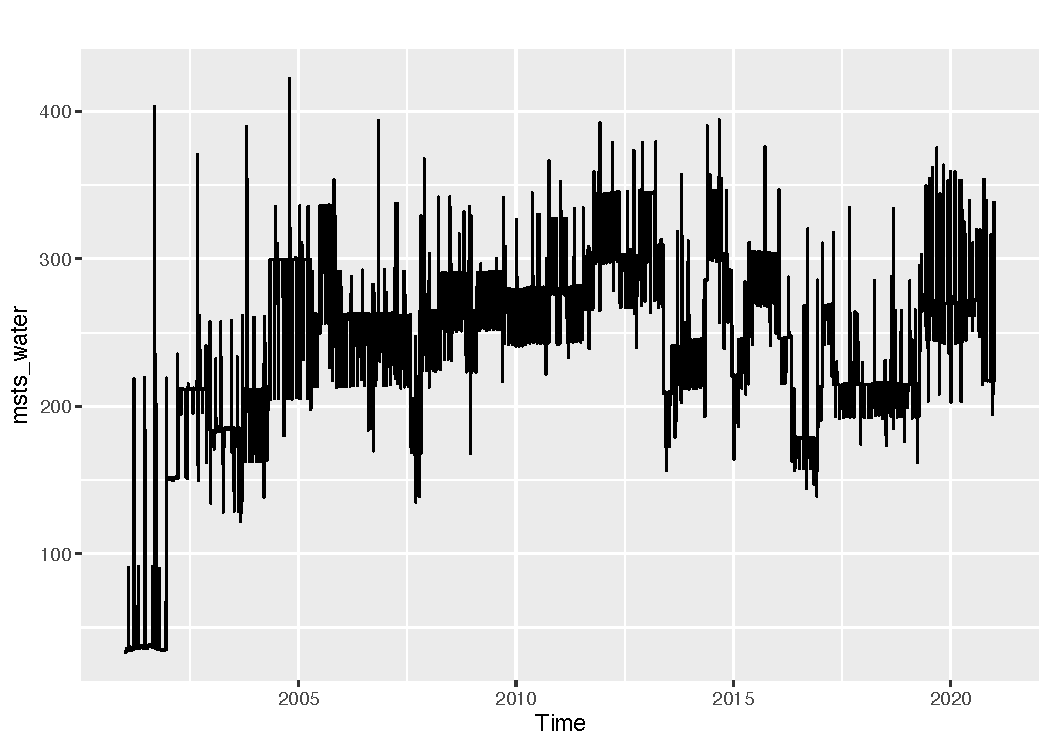
\includegraphics{Sai_files/figure-latex/Create time series object-1} \end{center}

\begin{Shaded}
\begin{Highlighting}[]
\CommentTok{\#question}
\end{Highlighting}
\end{Shaded}

\begin{Shaded}
\begin{Highlighting}[]
\CommentTok{\#ts\_water\_monthly\textless{}{-}ts(df\_water\_monthly[,2], frequency=12,start =c(2010,01), end=c(2021,10))}

\CommentTok{\#water}
\FunctionTok{par}\NormalTok{(}\AttributeTok{mfrow=}\FunctionTok{c}\NormalTok{(}\DecValTok{1}\NormalTok{,}\DecValTok{2}\NormalTok{))}
\FunctionTok{Acf}\NormalTok{(ts\_water\_monthly,}\AttributeTok{lag.max=}\DecValTok{40}\NormalTok{,}\AttributeTok{main=}\FunctionTok{paste}\NormalTok{(}\StringTok{"ACF for Groundwater"}\NormalTok{),}\AttributeTok{ylim=}\FunctionTok{c}\NormalTok{(}\SpecialCharTok{{-}}\FloatTok{0.5}\NormalTok{,}\DecValTok{1}\NormalTok{)) }
\FunctionTok{Pacf}\NormalTok{(ts\_water\_monthly,}\AttributeTok{lag.max=}\DecValTok{40}\NormalTok{,}\AttributeTok{main=}\FunctionTok{paste}\NormalTok{(}\StringTok{"PACF for Groundwater"}\NormalTok{),}\AttributeTok{ylim=}\FunctionTok{c}\NormalTok{(}\SpecialCharTok{{-}}\FloatTok{0.5}\NormalTok{,}\DecValTok{1}\NormalTok{))}
\end{Highlighting}
\end{Shaded}

\begin{center}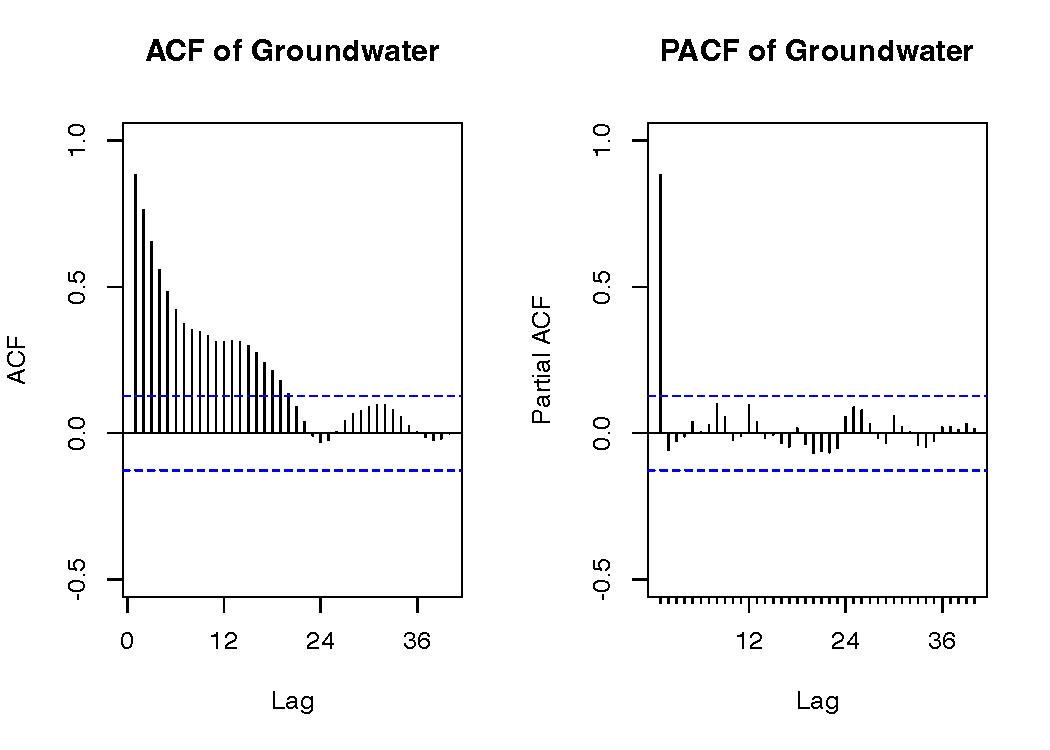
\includegraphics{Sai_files/figure-latex/ACF and PACF-1} \end{center}

\begin{Shaded}
\begin{Highlighting}[]
\FunctionTok{plot\_grid}\NormalTok{(}
  \FunctionTok{autoplot}\NormalTok{(ts\_water\_monthly),}
  \FunctionTok{autoplot}\NormalTok{(}\FunctionTok{Acf}\NormalTok{(ts\_water\_monthly,}\AttributeTok{plot=}\ConstantTok{FALSE}\NormalTok{,}\AttributeTok{lag.max=}\DecValTok{40}\NormalTok{)),}
  \FunctionTok{autoplot}\NormalTok{(}\FunctionTok{Pacf}\NormalTok{(ts\_water\_monthly,}\AttributeTok{plot=}\ConstantTok{FALSE}\NormalTok{,}\AttributeTok{lag.max=}\DecValTok{40}\NormalTok{)),}
  \AttributeTok{nrow=}\DecValTok{1}
\NormalTok{)}
\end{Highlighting}
\end{Shaded}

\begin{center}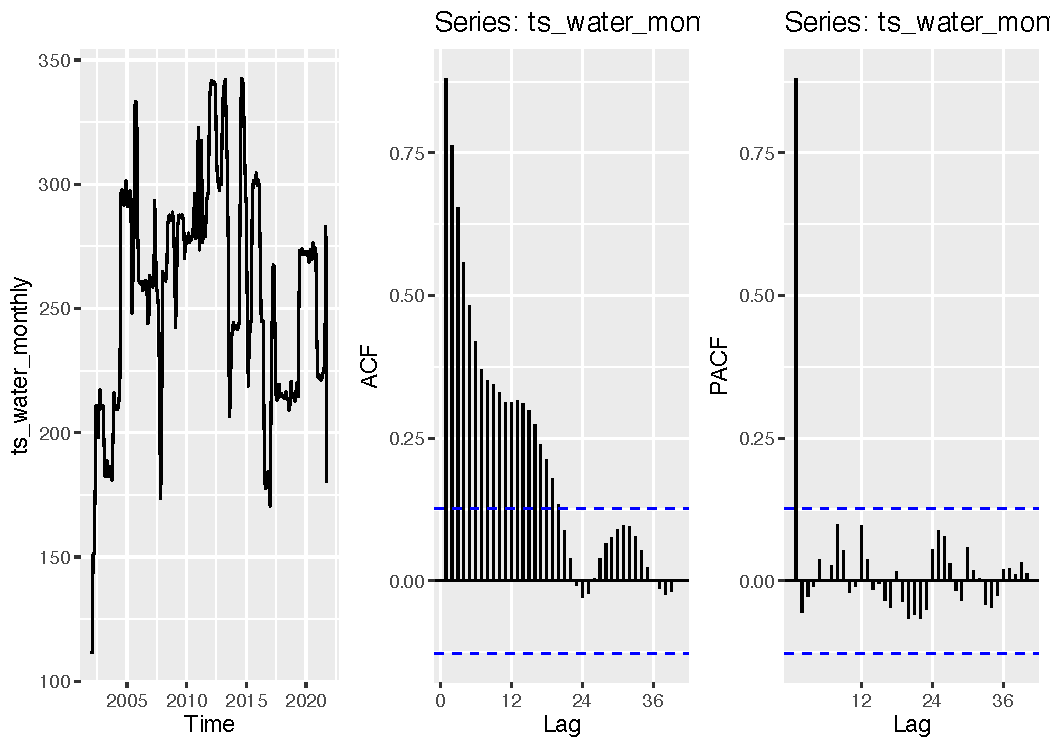
\includegraphics{Sai_files/figure-latex/ACF and PACF-2} \end{center}

\begin{Shaded}
\begin{Highlighting}[]
\CommentTok{\#decompose }
\NormalTok{water\_decompose}\OtherTok{\textless{}{-}}\FunctionTok{decompose}\NormalTok{(ts\_water\_monthly)}
\FunctionTok{plot}\NormalTok{(water\_decompose)}
\end{Highlighting}
\end{Shaded}

\begin{center}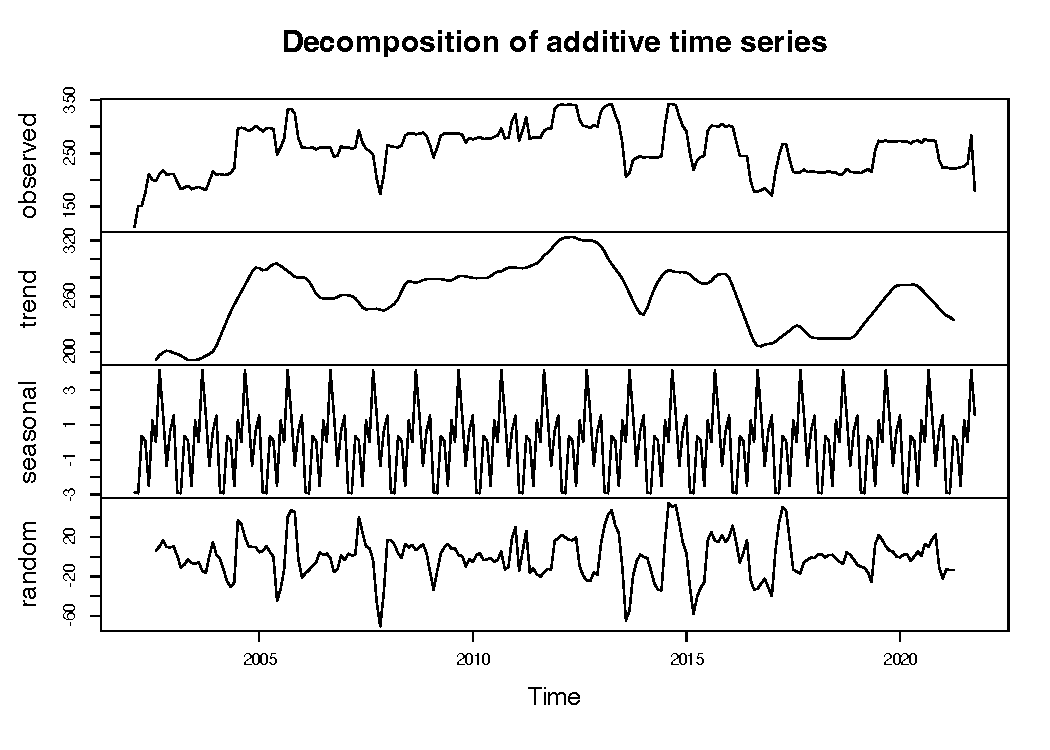
\includegraphics{Sai_files/figure-latex/Detrend and deseason-1} \end{center}

\begin{Shaded}
\begin{Highlighting}[]
\CommentTok{\#deseason}
\NormalTok{water\_deseason}\OtherTok{\textless{}{-}}\FunctionTok{seasadj}\NormalTok{(water\_decompose)}
\FunctionTok{plot\_grid}\NormalTok{(}
  \FunctionTok{autoplot}\NormalTok{(water\_deseason),}
  \FunctionTok{autoplot}\NormalTok{(}\FunctionTok{Acf}\NormalTok{(water\_deseason,}\AttributeTok{plot=}\ConstantTok{FALSE}\NormalTok{,}\AttributeTok{lag.max=}\DecValTok{40}\NormalTok{)),}
  \FunctionTok{autoplot}\NormalTok{(}\FunctionTok{Pacf}\NormalTok{(water\_deseason,}\AttributeTok{plot=}\ConstantTok{FALSE}\NormalTok{,}\AttributeTok{lag.max=}\DecValTok{40}\NormalTok{)),}
  \AttributeTok{nrow=}\DecValTok{1}
\NormalTok{)}
\end{Highlighting}
\end{Shaded}

\begin{center}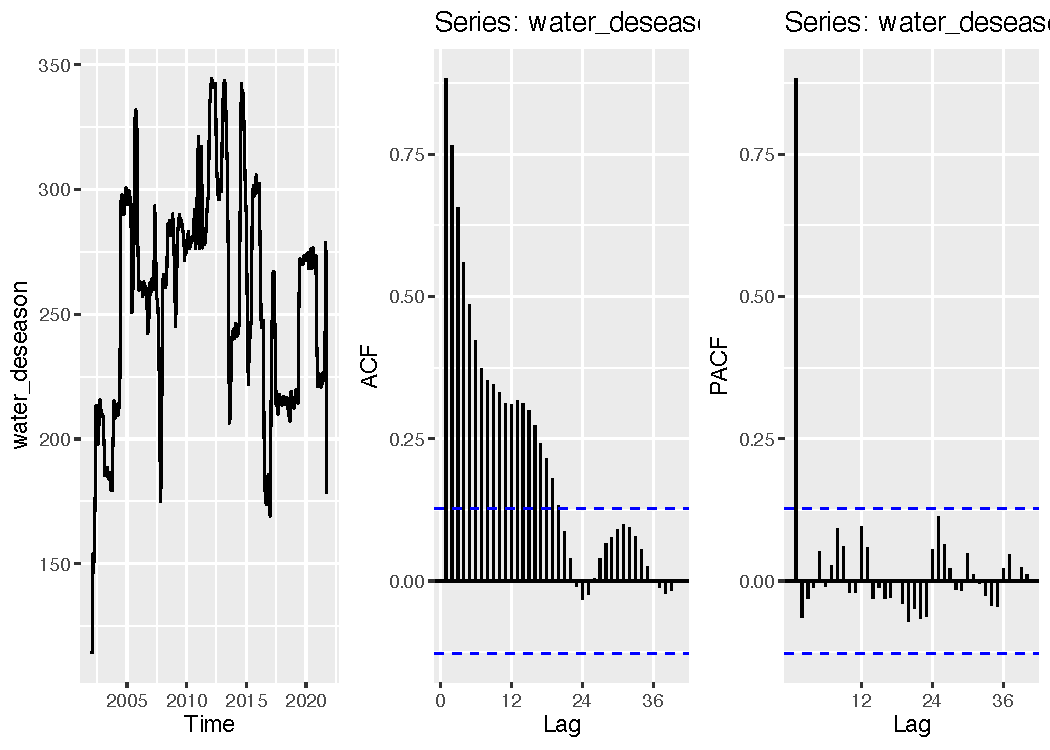
\includegraphics{Sai_files/figure-latex/Detrend and deseason-2} \end{center}

\begin{Shaded}
\begin{Highlighting}[]
\FunctionTok{par}\NormalTok{(}\AttributeTok{mfrow=}\FunctionTok{c}\NormalTok{(}\DecValTok{1}\NormalTok{,}\DecValTok{2}\NormalTok{))}
\FunctionTok{Acf}\NormalTok{(water\_deseason,}\AttributeTok{lag.max=}\DecValTok{40}\NormalTok{,}\AttributeTok{main=}\FunctionTok{paste}\NormalTok{(}\StringTok{"ACF for Groundwater"}\NormalTok{),}\AttributeTok{ylim=}\FunctionTok{c}\NormalTok{(}\SpecialCharTok{{-}}\FloatTok{0.5}\NormalTok{,}\DecValTok{1}\NormalTok{)) }
\FunctionTok{Pacf}\NormalTok{(water\_deseason,}\AttributeTok{lag.max=}\DecValTok{40}\NormalTok{,}\AttributeTok{main=}\FunctionTok{paste}\NormalTok{(}\StringTok{"PACF for Groundwater"}\NormalTok{),}\AttributeTok{ylim=}\FunctionTok{c}\NormalTok{(}\SpecialCharTok{{-}}\FloatTok{0.5}\NormalTok{,}\DecValTok{1}\NormalTok{))}
\end{Highlighting}
\end{Shaded}

\begin{center}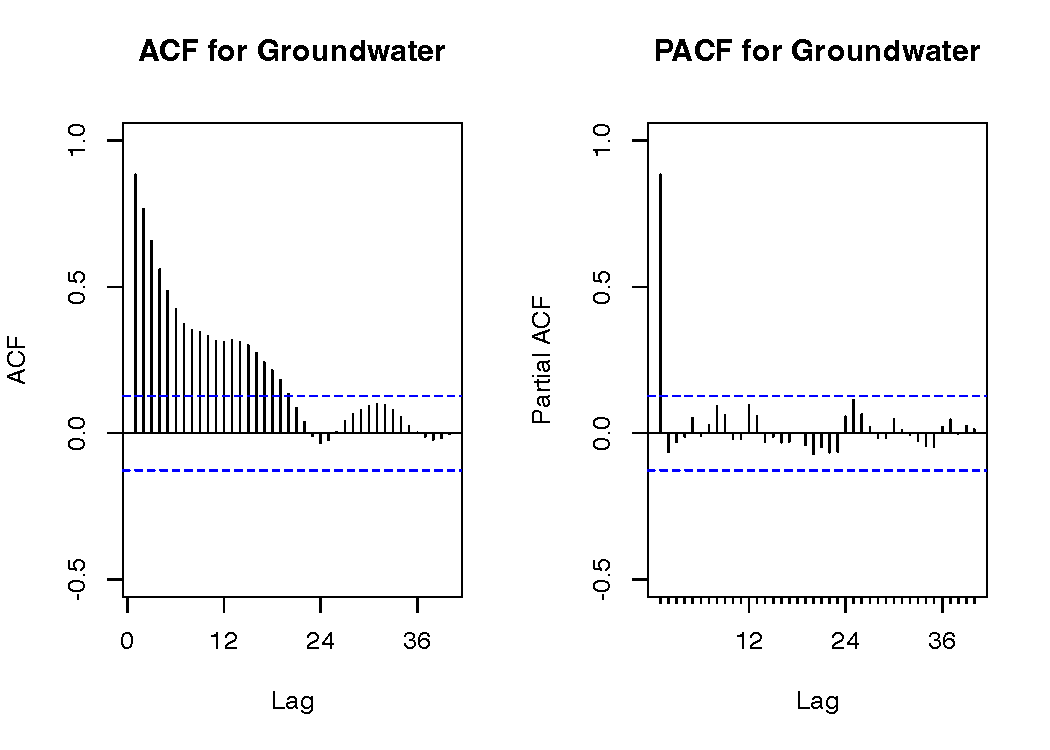
\includegraphics{Sai_files/figure-latex/Detrend and deseason-3} \end{center}

\begin{Shaded}
\begin{Highlighting}[]
\CommentTok{\#ts; monthly }
\CommentTok{\#Mann{-}Kendall}
\FunctionTok{summary}\NormalTok{(}\FunctionTok{MannKendall}\NormalTok{(water\_deseason)) }\CommentTok{\#reject the null hypothesis, supporting the presence of a trend}
\end{Highlighting}
\end{Shaded}

\begin{verbatim}
## Score =  808 , Var(Score) = 1488413
## denominator =  27966
## tau = 0.0289, 2-sided pvalue =0.50831
\end{verbatim}

\begin{Shaded}
\begin{Highlighting}[]
\CommentTok{\#seasonal Mann{-}Kendall}
\CommentTok{\#correction: calculate monthly average }
\NormalTok{trend}\SpecialCharTok{::}\FunctionTok{smk.test}\NormalTok{(water\_deseason) }
\end{Highlighting}
\end{Shaded}

\begin{verbatim}
## 
##  Seasonal Mann-Kendall trend test (Hirsch-Slack test)
## 
## data:  water_deseason
## z = 0.53391, p-value = 0.5934
## alternative hypothesis: true S is not equal to 0
## sample estimates:
##     S  varS 
##    57 11001
\end{verbatim}

\begin{Shaded}
\begin{Highlighting}[]
\CommentTok{\#ADF test}
\FunctionTok{print}\NormalTok{(}\FunctionTok{adf.test}\NormalTok{(water\_deseason,}\AttributeTok{alternative =} \StringTok{"stationary"}\NormalTok{)) }\CommentTok{\#reject the null hypothesis, the trend is stationary }
\end{Highlighting}
\end{Shaded}

\begin{verbatim}
## 
##  Augmented Dickey-Fuller Test
## 
## data:  water_deseason
## Dickey-Fuller = -3.0006, Lag order = 6, p-value = 0.1552
## alternative hypothesis: stationary
\end{verbatim}

\begin{Shaded}
\begin{Highlighting}[]
\CommentTok{\#not sure why we are running it on deseasoned data here since this test can handle seasonality}

\FunctionTok{print}\NormalTok{(}\FunctionTok{adf.test}\NormalTok{(ts\_water\_monthly,}\AttributeTok{alternative =} \StringTok{"stationary"}\NormalTok{))}
\end{Highlighting}
\end{Shaded}

\begin{verbatim}
## 
##  Augmented Dickey-Fuller Test
## 
## data:  ts_water_monthly
## Dickey-Fuller = -3.0442, Lag order = 6, p-value = 0.1368
## alternative hypothesis: stationary
\end{verbatim}

\begin{Shaded}
\begin{Highlighting}[]
\CommentTok{\#p{-}value\textgreater{}0.05 so null hypothesis cant be rejected and trend is stochastic}

\NormalTok{SMKtest}\OtherTok{\textless{}{-}} \FunctionTok{SeasonalMannKendall}\NormalTok{(ts\_water\_monthly)}
\FunctionTok{print}\NormalTok{(}\FunctionTok{summary}\NormalTok{(SMKtest))}
\end{Highlighting}
\end{Shaded}

\begin{verbatim}
## Score =  57 , Var(Score) = 11001
## denominator =  2223
## tau = 0.0256, 2-sided pvalue =0.58682
## NULL
\end{verbatim}

\begin{Shaded}
\begin{Highlighting}[]
\CommentTok{\#ts; monthly}
\CommentTok{\#find out how many times is needed for differencing }
\CommentTok{\#ns\_diff\textless{}{-}nsdiffs(water\_deseason)}
\CommentTok{\#cat("Number of seasonal differencing needed:", ns\_diff) \#no need to difference the series}
\CommentTok{\#question: does not need to difference the series but has trend in the data}

\CommentTok{\#this is no need for seasonal differencing}

\NormalTok{n\_diff}\OtherTok{\textless{}{-}} \FunctionTok{ndiffs}\NormalTok{(ts\_water\_monthly)}
\FunctionTok{cat}\NormalTok{(}\StringTok{"Number of trend differencing needed:"}\NormalTok{, n\_diff)}
\end{Highlighting}
\end{Shaded}

\begin{verbatim}
## Number of trend differencing needed: 1
\end{verbatim}

\begin{Shaded}
\begin{Highlighting}[]
\CommentTok{\#differencing is still needed for the stationary trend, d=1}
\end{Highlighting}
\end{Shaded}

\begin{Shaded}
\begin{Highlighting}[]
\CommentTok{\#water}
\CommentTok{\#from 2001{-}03{-}01 to 2021{-}10{-}22}

\CommentTok{\#monthly ts}
\CommentTok{\#ts\_training\textless{}{-}ts(df\_water\_monthly[,2],}
                \CommentTok{\#frequency=12,}
                \CommentTok{\#start=c(2002,02), end=c(2020,09))}

\CommentTok{\#I\textquotesingle{}m not sure why the start=c(2010,01) says 2010. Shouldn\textquotesingle{}t it be 2001?}


\CommentTok{\#ts\_testing\textless{}{-}ts(df\_water\_monthly[,2],}
               \CommentTok{\#frequency=12,}
               \CommentTok{\#start=c(2020,10), end=c(2021,10))}

\NormalTok{nobs }\OtherTok{\textless{}{-}} \FunctionTok{nrow}\NormalTok{(df\_water\_monthly)}
\NormalTok{nfor }\OtherTok{\textless{}{-}} \DecValTok{12}

\NormalTok{ts\_training2 }\OtherTok{\textless{}{-}} \FunctionTok{subset}\NormalTok{(ts\_water\_monthly, }\AttributeTok{end=}\FunctionTok{length}\NormalTok{(ts\_water\_monthly)}\SpecialCharTok{{-}}\NormalTok{nfor)}
\NormalTok{ts\_testing2 }\OtherTok{\textless{}{-}} \FunctionTok{subset}\NormalTok{(ts\_water\_monthly, }\AttributeTok{start =} \FunctionTok{length}\NormalTok{(ts\_water\_monthly)}\SpecialCharTok{{-}}\NormalTok{nfor}\SpecialCharTok{+}\DecValTok{1}\NormalTok{)}

\FunctionTok{autoplot}\NormalTok{(ts\_training2)}
\end{Highlighting}
\end{Shaded}

\begin{center}\includegraphics{Sai_files/figure-latex/Training and testing-1} \end{center}

\begin{Shaded}
\begin{Highlighting}[]
\FunctionTok{autoplot}\NormalTok{(ts\_testing2)}
\end{Highlighting}
\end{Shaded}

\begin{center}\includegraphics{Sai_files/figure-latex/Training and testing-2} \end{center}

\begin{Shaded}
\begin{Highlighting}[]
\CommentTok{\#ts(ts\_water\_monthly[1:(nobs{-}nfor)],}
\CommentTok{\#start=c(2002,02),}
\CommentTok{\#frequency = 12)}
  
\CommentTok{\#ts\_water\_monthly[(nobs{-}nfor+1):nobs]}
\CommentTok{\#head(ts\_testing2)}
\end{Highlighting}
\end{Shaded}

\begin{Shaded}
\begin{Highlighting}[]
\FunctionTok{par}\NormalTok{(}\AttributeTok{mfrow=}\FunctionTok{c}\NormalTok{(}\DecValTok{1}\NormalTok{,}\DecValTok{1}\NormalTok{))}

\CommentTok{\#SARIMA}

\NormalTok{sarima\_fit }\OtherTok{\textless{}{-}} \FunctionTok{auto.arima}\NormalTok{(ts\_training2)}
\FunctionTok{checkresiduals}\NormalTok{(sarima\_fit)}
\end{Highlighting}
\end{Shaded}

\begin{center}\includegraphics{Sai_files/figure-latex/unnamed-chunk-2-1} \end{center}

\begin{verbatim}
## 
##  Ljung-Box test
## 
## data:  Residuals from ARIMA(1,1,2)
## Q* = 20.844, df = 21, p-value = 0.4685
## 
## Model df: 3.   Total lags used: 24
\end{verbatim}

\begin{Shaded}
\begin{Highlighting}[]
\NormalTok{sarima\_for }\OtherTok{\textless{}{-}} \FunctionTok{forecast}\NormalTok{(sarima\_fit,}\AttributeTok{h=}\NormalTok{nfor)}
\FunctionTok{plot}\NormalTok{(sarima\_for)}
\end{Highlighting}
\end{Shaded}

\begin{center}\includegraphics{Sai_files/figure-latex/unnamed-chunk-2-2} \end{center}

\begin{Shaded}
\begin{Highlighting}[]
\NormalTok{sarima\_score }\OtherTok{\textless{}{-}} \FunctionTok{accuracy}\NormalTok{(sarima\_for}\SpecialCharTok{$}\NormalTok{mean, ts\_testing2)}
\end{Highlighting}
\end{Shaded}

\begin{Shaded}
\begin{Highlighting}[]
\NormalTok{ETS\_fit }\OtherTok{\textless{}{-}} \FunctionTok{stlf}\NormalTok{(ts\_training2,}\AttributeTok{h=}\NormalTok{nfor)}

\NormalTok{ETS\_score }\OtherTok{\textless{}{-}} \FunctionTok{accuracy}\NormalTok{(ETS\_fit}\SpecialCharTok{$}\NormalTok{mean, ts\_testing2)}

\FunctionTok{autoplot}\NormalTok{(ts\_water\_monthly)}\SpecialCharTok{+}
  \FunctionTok{autolayer}\NormalTok{(ETS\_fit, }\AttributeTok{series=}\StringTok{"STL +ETS"}\NormalTok{, }\AttributeTok{PI=}\ConstantTok{FALSE}\NormalTok{)}\SpecialCharTok{+}
  \FunctionTok{autolayer}\NormalTok{(sarima\_for, }\AttributeTok{series =} \StringTok{"SARIMA"}\NormalTok{, }\AttributeTok{PI=}\ConstantTok{FALSE}\NormalTok{)}
\end{Highlighting}
\end{Shaded}

\begin{center}\includegraphics{Sai_files/figure-latex/ETS-1} \end{center}

\begin{Shaded}
\begin{Highlighting}[]
\NormalTok{SS\_ll }\OtherTok{\textless{}{-}} \FunctionTok{StructTS}\NormalTok{(ts\_training2, }\AttributeTok{type=}\StringTok{"level"}\NormalTok{)}
\NormalTok{SS\_llt }\OtherTok{\textless{}{-}} \FunctionTok{StructTS}\NormalTok{(ts\_training2, }\AttributeTok{type=}\StringTok{"trend"}\NormalTok{)}
\NormalTok{SS\_bsm }\OtherTok{\textless{}{-}} \FunctionTok{StructTS}\NormalTok{(ts\_training2, }\AttributeTok{type=}\StringTok{"BSM"}\NormalTok{)}

\NormalTok{SS\_ll\_for }\OtherTok{\textless{}{-}} \FunctionTok{forecast}\NormalTok{(SS\_ll,}\AttributeTok{h=}\NormalTok{nfor)}
\FunctionTok{plot}\NormalTok{(SS\_ll\_for)}
\end{Highlighting}
\end{Shaded}

\begin{center}\includegraphics{Sai_files/figure-latex/SS-1} \end{center}

\begin{Shaded}
\begin{Highlighting}[]
\NormalTok{SS\_ll\_score }\OtherTok{\textless{}{-}} \FunctionTok{accuracy}\NormalTok{(SS\_ll\_for}\SpecialCharTok{$}\NormalTok{mean,ts\_testing2)}

\NormalTok{SS\_llt\_for }\OtherTok{\textless{}{-}} \FunctionTok{forecast}\NormalTok{(SS\_llt,}\AttributeTok{h=}\NormalTok{nfor)}
\FunctionTok{plot}\NormalTok{(SS\_llt\_for)}
\end{Highlighting}
\end{Shaded}

\begin{center}\includegraphics{Sai_files/figure-latex/SS-2} \end{center}

\begin{Shaded}
\begin{Highlighting}[]
\NormalTok{SS\_llt\_score }\OtherTok{\textless{}{-}} \FunctionTok{accuracy}\NormalTok{(SS\_llt\_for}\SpecialCharTok{$}\NormalTok{mean,ts\_testing2)}

\NormalTok{SS\_bsm\_for }\OtherTok{\textless{}{-}} \FunctionTok{forecast}\NormalTok{(SS\_bsm,}\AttributeTok{h=}\NormalTok{nfor)}
\FunctionTok{plot}\NormalTok{(SS\_bsm\_for)}
\end{Highlighting}
\end{Shaded}

\begin{center}\includegraphics{Sai_files/figure-latex/SS-3} \end{center}

\begin{Shaded}
\begin{Highlighting}[]
\NormalTok{SS\_bsm\_score }\OtherTok{\textless{}{-}} \FunctionTok{accuracy}\NormalTok{(SS\_bsm\_for}\SpecialCharTok{$}\NormalTok{mean,ts\_testing2)}

\CommentTok{\#ETS is better if looking at MAPE}
\end{Highlighting}
\end{Shaded}

\begin{Shaded}
\begin{Highlighting}[]
\CommentTok{\#ARIMA +Fourier}
\NormalTok{ARIMA\_Four\_fit\_1}\OtherTok{\textless{}{-}}\FunctionTok{auto.arima}\NormalTok{(ts\_training2,}
                             \AttributeTok{seasonal=}\ConstantTok{FALSE}\NormalTok{, }
                             \AttributeTok{xreg=}\FunctionTok{fourier}\NormalTok{(ts\_training2,}\AttributeTok{K=}\FunctionTok{c}\NormalTok{(}\DecValTok{2}\NormalTok{)))}
\CommentTok{\#forecast with ARIMA\_fit}
\NormalTok{ARIMA\_Four\_forecast\_1}\OtherTok{\textless{}{-}}\FunctionTok{forecast}\NormalTok{(ARIMA\_Four\_fit\_1,}
                                \AttributeTok{xreg=}\FunctionTok{fourier}\NormalTok{(ts\_training2,}\AttributeTok{K=}\FunctionTok{c}\NormalTok{(}\DecValTok{2}\NormalTok{),}\AttributeTok{h=}\NormalTok{nfor),}
                                \AttributeTok{h=}\NormalTok{nfor) }

\CommentTok{\#K=c(4)}
\NormalTok{ARIMA\_Four\_fit\_2}\OtherTok{\textless{}{-}}\FunctionTok{auto.arima}\NormalTok{(ts\_training2,}
                             \AttributeTok{seasonal=}\ConstantTok{FALSE}\NormalTok{, }
                             \AttributeTok{xreg=}\FunctionTok{fourier}\NormalTok{(ts\_training2,}\AttributeTok{K=}\FunctionTok{c}\NormalTok{(}\DecValTok{4}\NormalTok{)))}
\CommentTok{\#forecast with ARIMA\_fit}
\NormalTok{ARIMA\_Four\_forecast\_2}\OtherTok{\textless{}{-}}\FunctionTok{forecast}\NormalTok{(ARIMA\_Four\_fit\_2,}
                                \AttributeTok{xreg=}\FunctionTok{fourier}\NormalTok{(ts\_training2,}\AttributeTok{K=}\FunctionTok{c}\NormalTok{(}\DecValTok{4}\NormalTok{),}\AttributeTok{h=}\NormalTok{nfor),}
                                \AttributeTok{h=}\NormalTok{nfor)}

\CommentTok{\#K=c(6)}
\NormalTok{ARIMA\_Four\_fit\_3}\OtherTok{\textless{}{-}}\FunctionTok{auto.arima}\NormalTok{(ts\_training2,}
                             \AttributeTok{seasonal=}\ConstantTok{FALSE}\NormalTok{, }
                             \AttributeTok{xreg=}\FunctionTok{fourier}\NormalTok{(ts\_training2,}\AttributeTok{K=}\FunctionTok{c}\NormalTok{(}\DecValTok{6}\NormalTok{)))}
\CommentTok{\#forecast with ARIMA\_fit}
\NormalTok{ARIMA\_Four\_forecast\_3}\OtherTok{\textless{}{-}}\FunctionTok{forecast}\NormalTok{(ARIMA\_Four\_fit\_3,}
                                \AttributeTok{xreg=}\FunctionTok{fourier}\NormalTok{(ts\_training2,}\AttributeTok{K=}\FunctionTok{c}\NormalTok{(}\DecValTok{6}\NormalTok{),}\AttributeTok{h=}\NormalTok{nfor),}
                                \AttributeTok{h=}\NormalTok{nfor)}

\NormalTok{scores\_ARIMA\_Four\_forecast\_1}\OtherTok{\textless{}{-}}\FunctionTok{accuracy}\NormalTok{(ARIMA\_Four\_forecast\_1}\SpecialCharTok{$}\NormalTok{mean,ts\_testing2)}
\NormalTok{scores\_ARIMA\_Four\_forecast\_2}\OtherTok{\textless{}{-}}\FunctionTok{accuracy}\NormalTok{(ARIMA\_Four\_forecast\_2}\SpecialCharTok{$}\NormalTok{mean,ts\_testing2)}
\NormalTok{scores\_ARIMA\_Four\_forecast\_3}\OtherTok{\textless{}{-}}\FunctionTok{accuracy}\NormalTok{(ARIMA\_Four\_forecast\_3}\SpecialCharTok{$}\NormalTok{mean,ts\_testing2)}
\end{Highlighting}
\end{Shaded}

\begin{Shaded}
\begin{Highlighting}[]
\CommentTok{\#temp}
\CommentTok{\#create time series object }
\CommentTok{\#ts\_temp\_training\textless{}{-}ts(df\_temp\_preci[,2], frequency=12,}
                     \CommentTok{\#start=c(2010,01), end=c(2020,09))}

\CommentTok{\#ts\_temp\_testing\textless{}{-}ts(df\_temp\_preci[,2], frequency=12,}
                     \CommentTok{\#start=c(2020,10), end=c(2021,10))}

\NormalTok{ts\_temp\_monthly}\OtherTok{\textless{}{-}}\FunctionTok{ts}\NormalTok{(df\_temp\_preci2[,}\DecValTok{2}\NormalTok{], }\AttributeTok{frequency=}\DecValTok{12}\NormalTok{,}\AttributeTok{start =}\FunctionTok{c}\NormalTok{(}\DecValTok{2002}\NormalTok{,}\DecValTok{02}\NormalTok{), }\AttributeTok{end=}\FunctionTok{c}\NormalTok{(}\DecValTok{2021}\NormalTok{,}\DecValTok{10}\NormalTok{))}
\NormalTok{ts\_preci\_monthly}\OtherTok{\textless{}{-}}\FunctionTok{ts}\NormalTok{(df\_temp\_preci2[,}\DecValTok{3}\NormalTok{], }\AttributeTok{frequency=}\DecValTok{12}\NormalTok{,}\AttributeTok{start =}\FunctionTok{c}\NormalTok{(}\DecValTok{2002}\NormalTok{,}\DecValTok{02}\NormalTok{), }\AttributeTok{end=}\FunctionTok{c}\NormalTok{(}\DecValTok{2021}\NormalTok{,}\DecValTok{10}\NormalTok{))}

\CommentTok{\#preci}
\CommentTok{\#create time series object }
\CommentTok{\#ts\_preci\_training\textless{}{-}ts(df\_temp\_preci[,3], frequency=12,}
                      \CommentTok{\#start=c(2010,01), end=c(2020,09))}

\CommentTok{\#ts\_preci\_testing\textless{}{-}ts(df\_temp\_preci[,3], frequency=12,}
                     \CommentTok{\#start=c(2020,10), end=c(2021,10))}

\CommentTok{\#ts\_temp\textless{}{-}ts(df\_temp\_preci[,2], frequency=12,start=c(2010,01), end=c(2021,10))}
\CommentTok{\#ts\_preci\textless{}{-}ts(df\_temp\_preci[,3], frequency=12,start=c(2010,01), end=c(2021,10))}

\FunctionTok{autoplot}\NormalTok{(ts\_temp\_monthly)}
\end{Highlighting}
\end{Shaded}

\begin{center}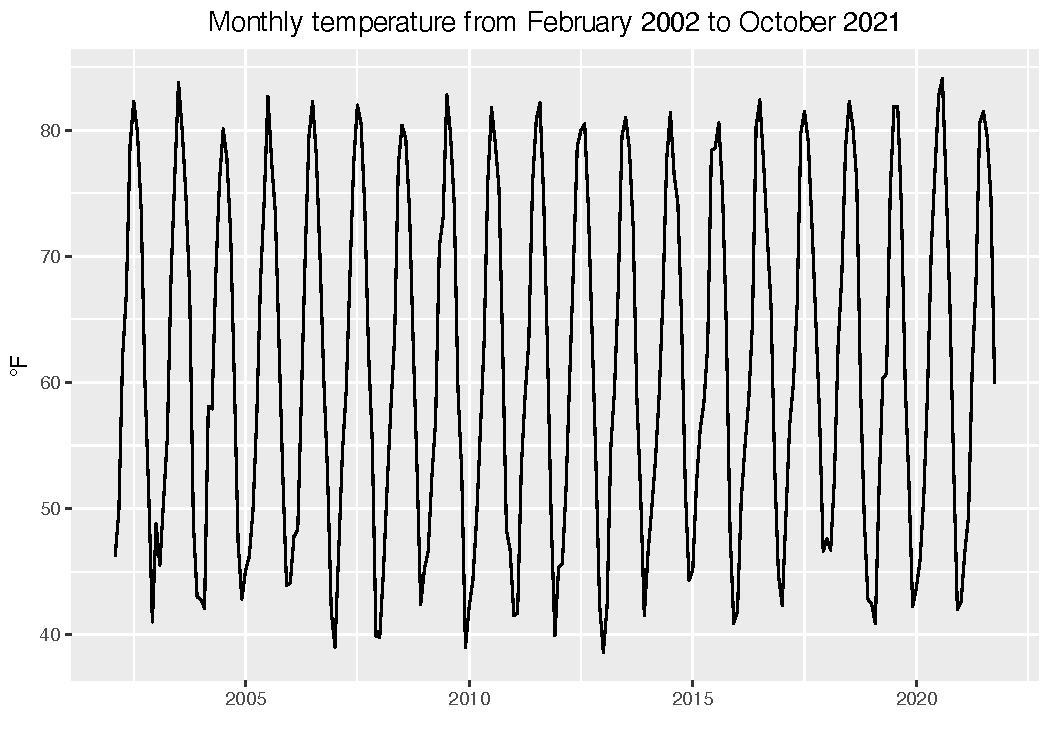
\includegraphics{Sai_files/figure-latex/exogenous variable-1} \end{center}

\begin{Shaded}
\begin{Highlighting}[]
\FunctionTok{autoplot}\NormalTok{(ts\_preci\_monthly)}
\end{Highlighting}
\end{Shaded}

\begin{center}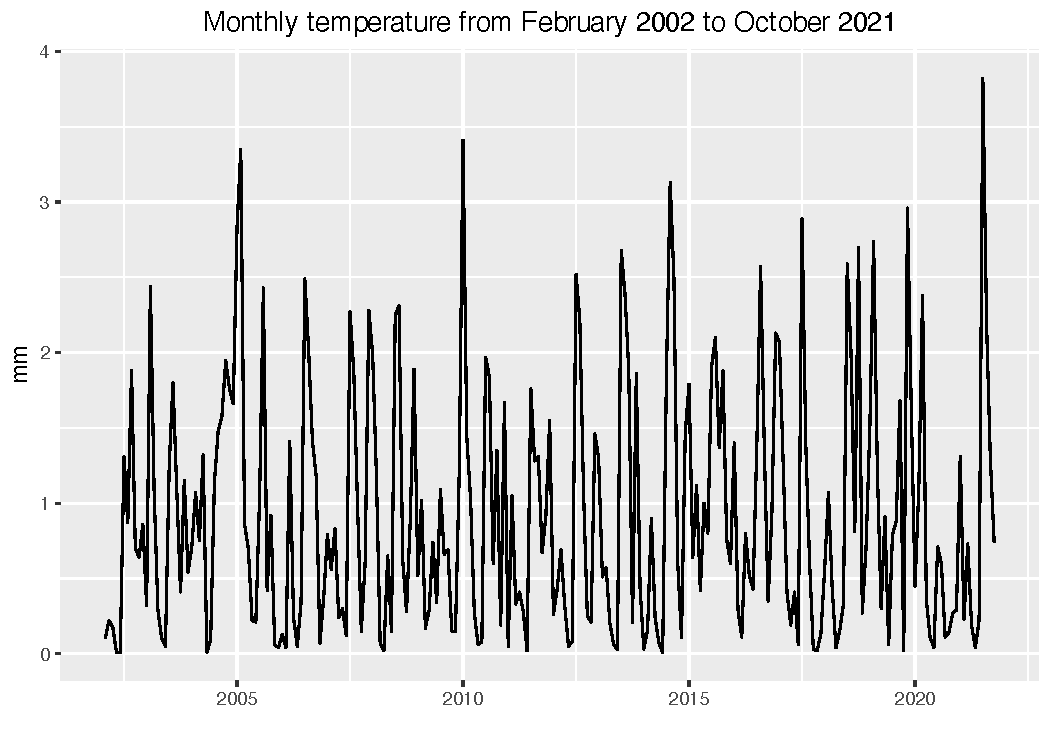
\includegraphics{Sai_files/figure-latex/exogenous variable-2} \end{center}

\begin{Shaded}
\begin{Highlighting}[]
\NormalTok{ts\_temp\_training2 }\OtherTok{\textless{}{-}} \FunctionTok{subset}\NormalTok{(ts\_temp\_monthly, }\AttributeTok{end=}\FunctionTok{length}\NormalTok{(ts\_temp\_monthly)}\SpecialCharTok{{-}}\NormalTok{nfor)}
\NormalTok{ts\_temp\_testing2 }\OtherTok{\textless{}{-}} \FunctionTok{subset}\NormalTok{(ts\_temp\_monthly, }\AttributeTok{start =} \FunctionTok{length}\NormalTok{(ts\_temp\_monthly)}\SpecialCharTok{{-}}\NormalTok{nfor}\SpecialCharTok{+}\DecValTok{1}\NormalTok{)}

\NormalTok{ts\_preci\_training2 }\OtherTok{\textless{}{-}} \FunctionTok{subset}\NormalTok{(ts\_preci\_monthly, }\AttributeTok{end=}\FunctionTok{length}\NormalTok{(ts\_preci\_monthly)}\SpecialCharTok{{-}}\NormalTok{nfor)}
\NormalTok{ts\_preci\_testing2 }\OtherTok{\textless{}{-}} \FunctionTok{subset}\NormalTok{(ts\_preci\_monthly, }\AttributeTok{start =} \FunctionTok{length}\NormalTok{(ts\_preci\_monthly)}\SpecialCharTok{{-}}\NormalTok{nfor}\SpecialCharTok{+}\DecValTok{1}\NormalTok{)}
\end{Highlighting}
\end{Shaded}

\begin{Shaded}
\begin{Highlighting}[]
\CommentTok{\#correlation test }
\NormalTok{cor\_water\_temp}\OtherTok{\textless{}{-}}\FunctionTok{cor.test}\NormalTok{(ts\_water\_monthly,ts\_temp\_monthly,}\AttributeTok{method =} \StringTok{"spearman"}\NormalTok{,}\AttributeTok{exact =} \ConstantTok{FALSE}\NormalTok{)}
\NormalTok{cor\_water\_preci}\OtherTok{\textless{}{-}}\FunctionTok{cor.test}\NormalTok{(ts\_water\_monthly,ts\_preci\_monthly,}\AttributeTok{method =} \StringTok{"spearman"}\NormalTok{,}\AttributeTok{exact =} \ConstantTok{FALSE}\NormalTok{)}


\CommentTok{\#create a summary table }
\NormalTok{summary\_table\_cor}\OtherTok{\textless{}{-}}\FunctionTok{data.frame}\NormalTok{(}
  \AttributeTok{Variable =} \FunctionTok{c}\NormalTok{(}\StringTok{"Temperature"}\NormalTok{, }\StringTok{"Precipitation"}\NormalTok{),}
  \AttributeTok{Correlation\_Coefficient =} \FunctionTok{round}\NormalTok{(}\FunctionTok{c}\NormalTok{(cor\_water\_temp}\SpecialCharTok{$}\NormalTok{estimate, }
\NormalTok{                                    cor\_water\_preci}\SpecialCharTok{$}\NormalTok{estimate), }\DecValTok{5}\NormalTok{),}
  \AttributeTok{P\_Value =} \FunctionTok{round}\NormalTok{(}\FunctionTok{c}\NormalTok{(cor\_water\_temp}\SpecialCharTok{$}\NormalTok{p.value, }
\NormalTok{                    cor\_water\_preci}\SpecialCharTok{$}\NormalTok{p.value), }\DecValTok{5}\NormalTok{)}
\NormalTok{)}

\FunctionTok{print}\NormalTok{(summary\_table\_cor)}
\end{Highlighting}
\end{Shaded}

\begin{verbatim}
##        Variable Correlation_Coefficient P_Value
## 1   Temperature                -0.00128 0.98438
## 2 Precipitation                 0.06314 0.33315
\end{verbatim}

\begin{Shaded}
\begin{Highlighting}[]
\CommentTok{\#decide not to use the exogenous variable }

\CommentTok{\#K=c(2)}
\CommentTok{\#fit ARIMA with deseason time series }

\NormalTok{xreg1 }\OtherTok{\textless{}{-}} \FunctionTok{as.matrix}\NormalTok{(}\FunctionTok{data.frame}\NormalTok{(}\FunctionTok{fourier}\NormalTok{(ts\_training2, }\AttributeTok{K=}\FunctionTok{c}\NormalTok{(}\DecValTok{2}\NormalTok{)),}\StringTok{"preci"}\OtherTok{=}\NormalTok{ts\_preci\_training2))}

\NormalTok{ARIMA\_Four\_fit\_XREG\_1}\OtherTok{\textless{}{-}}\FunctionTok{auto.arima}\NormalTok{(ts\_training2,}
                                  \AttributeTok{seasonal=}\ConstantTok{FALSE}\NormalTok{,}
                                  \CommentTok{\#combine fourier and exogenous variable time series  }
                                  \AttributeTok{xreg=}\NormalTok{xreg1) }

\CommentTok{\#generate fourier terms}
\CommentTok{\#fourier\_terms\_1\textless{}{-}fourier(ts\_training2, K=c(2), h=12)}
\CommentTok{\#generate forecast}
\NormalTok{preci\_forecast\_1}\OtherTok{\textless{}{-}}\FunctionTok{forecast}\NormalTok{(ts\_preci\_training2, }\AttributeTok{h=}\DecValTok{12}\NormalTok{)}
\CommentTok{\#combine fourier terms and forecasts into a numeric matrix}
\NormalTok{xreg1\_for}\OtherTok{\textless{}{-}}\FunctionTok{as.matrix}\NormalTok{(}\FunctionTok{data.frame}\NormalTok{(}\FunctionTok{fourier}\NormalTok{(ts\_training2, }\AttributeTok{K=}\FunctionTok{c}\NormalTok{(}\DecValTok{2}\NormalTok{), }\AttributeTok{h=}\DecValTok{12}\NormalTok{), }\StringTok{"preci"}\OtherTok{=}\NormalTok{preci\_forecast\_1}\SpecialCharTok{$}\NormalTok{mean))}

\CommentTok{\#forecast with ARIMA\_fit\_XREG}
\NormalTok{ARIMA\_Four\_forecast\_XREG\_1}\OtherTok{\textless{}{-}}\FunctionTok{forecast}\NormalTok{(ARIMA\_Four\_fit\_XREG\_1,}
                                     \AttributeTok{xreg=}\NormalTok{xreg1\_for,}
                                     \AttributeTok{h=}\DecValTok{12}\NormalTok{)}


\CommentTok{\#K=c(4)}

\NormalTok{xreg2 }\OtherTok{\textless{}{-}} \FunctionTok{as.matrix}\NormalTok{(}\FunctionTok{data.frame}\NormalTok{(}\FunctionTok{fourier}\NormalTok{(ts\_training2, }\AttributeTok{K=}\FunctionTok{c}\NormalTok{(}\DecValTok{4}\NormalTok{)),}\StringTok{"preci"}\OtherTok{=}\NormalTok{ts\_preci\_training2))}

\NormalTok{ARIMA\_Four\_fit\_XREG\_2}\OtherTok{\textless{}{-}}\FunctionTok{auto.arima}\NormalTok{(ts\_training2,}
                                  \AttributeTok{seasonal=}\ConstantTok{FALSE}\NormalTok{,}
                                  \CommentTok{\#combine fourier and exogenous variable time series  }
                                  \AttributeTok{xreg=}\NormalTok{xreg2) }

\CommentTok{\#generate fourier terms}
\CommentTok{\#fourier\_terms\_1\textless{}{-}fourier(ts\_training2, K=c(2), h=12)}
\CommentTok{\#generate forecast}
\NormalTok{preci\_forecast\_2}\OtherTok{\textless{}{-}}\FunctionTok{forecast}\NormalTok{(ts\_preci\_training2, }\AttributeTok{h=}\DecValTok{12}\NormalTok{)}
\CommentTok{\#combine fourier terms and forecasts into a numeric matrix}
\NormalTok{xreg2\_for}\OtherTok{\textless{}{-}}\FunctionTok{as.matrix}\NormalTok{(}\FunctionTok{data.frame}\NormalTok{(}\FunctionTok{fourier}\NormalTok{(ts\_training2, }\AttributeTok{K=}\FunctionTok{c}\NormalTok{(}\DecValTok{4}\NormalTok{), }\AttributeTok{h=}\DecValTok{12}\NormalTok{), }\StringTok{"preci"}\OtherTok{=}\NormalTok{preci\_forecast\_2}\SpecialCharTok{$}\NormalTok{mean))}

\CommentTok{\#forecast with ARIMA\_fit\_XREG}
\NormalTok{ARIMA\_Four\_forecast\_XREG\_2}\OtherTok{\textless{}{-}}\FunctionTok{forecast}\NormalTok{(ARIMA\_Four\_fit\_XREG\_2,}
                                     \AttributeTok{xreg=}\NormalTok{xreg2\_for,}
                                     \AttributeTok{h=}\DecValTok{12}\NormalTok{)}

\CommentTok{\#K=c(6)}
\NormalTok{xreg3 }\OtherTok{\textless{}{-}} \FunctionTok{as.matrix}\NormalTok{(}\FunctionTok{data.frame}\NormalTok{(}\FunctionTok{fourier}\NormalTok{(ts\_training2, }\AttributeTok{K=}\FunctionTok{c}\NormalTok{(}\DecValTok{6}\NormalTok{)),}\StringTok{"preci"}\OtherTok{=}\NormalTok{ts\_preci\_training2))}

\NormalTok{ARIMA\_Four\_fit\_XREG\_3}\OtherTok{\textless{}{-}}\FunctionTok{auto.arima}\NormalTok{(ts\_training2,}
                                  \AttributeTok{seasonal=}\ConstantTok{FALSE}\NormalTok{,}
                                  \CommentTok{\#combine fourier and exogenous variable time series  }
                                  \AttributeTok{xreg=}\NormalTok{xreg3) }

\CommentTok{\#generate fourier terms}
\CommentTok{\#fourier\_terms\_1\textless{}{-}fourier(ts\_training2, K=c(2), h=12)}
\CommentTok{\#generate forecast}
\NormalTok{preci\_forecast\_3}\OtherTok{\textless{}{-}}\FunctionTok{forecast}\NormalTok{(ts\_preci\_training2, }\AttributeTok{h=}\DecValTok{12}\NormalTok{)}
\CommentTok{\#combine fourier terms and forecasts into a numeric matrix}
\NormalTok{xreg3\_for}\OtherTok{\textless{}{-}}\FunctionTok{as.matrix}\NormalTok{(}\FunctionTok{data.frame}\NormalTok{(}\FunctionTok{fourier}\NormalTok{(ts\_training2, }\AttributeTok{K=}\FunctionTok{c}\NormalTok{(}\DecValTok{6}\NormalTok{), }\AttributeTok{h=}\DecValTok{12}\NormalTok{), }\StringTok{"preci"}\OtherTok{=}\NormalTok{preci\_forecast\_3}\SpecialCharTok{$}\NormalTok{mean))}

\CommentTok{\#forecast with ARIMA\_fit\_XREG}
\NormalTok{ARIMA\_Four\_forecast\_XREG\_3}\OtherTok{\textless{}{-}}\FunctionTok{forecast}\NormalTok{(ARIMA\_Four\_fit\_XREG\_3,}
                                     \AttributeTok{xreg=}\NormalTok{xreg3\_for,}
                                     \AttributeTok{h=}\DecValTok{12}\NormalTok{)}

 
\NormalTok{ARIMA\_Four\_XREG\_1\_score}\OtherTok{\textless{}{-}}\FunctionTok{accuracy}\NormalTok{(ARIMA\_Four\_forecast\_XREG\_1}\SpecialCharTok{$}\NormalTok{mean,ts\_testing2)}
\NormalTok{ARIMA\_Four\_XREG\_2\_score}\OtherTok{\textless{}{-}}\FunctionTok{accuracy}\NormalTok{(ARIMA\_Four\_forecast\_XREG\_2}\SpecialCharTok{$}\NormalTok{mean,ts\_testing2)}
\NormalTok{ARIMA\_Four\_XREG\_3\_score}\OtherTok{\textless{}{-}}\FunctionTok{accuracy}\NormalTok{(ARIMA\_Four\_forecast\_XREG\_3}\SpecialCharTok{$}\NormalTok{mean,ts\_testing2)}
\end{Highlighting}
\end{Shaded}

\begin{Shaded}
\begin{Highlighting}[]
\CommentTok{\#p=1, P=0 because seasonal=FALSE}

\CommentTok{\#K=c(2)}
\NormalTok{NN\_fit\_1}\OtherTok{\textless{}{-}}\FunctionTok{nnetar}\NormalTok{(ts\_training2,}
                 \AttributeTok{p=}\DecValTok{1}\NormalTok{,}
                 \AttributeTok{P=}\DecValTok{0}\NormalTok{,}
                 \AttributeTok{xreg=}\FunctionTok{fourier}\NormalTok{(ts\_training2,}\AttributeTok{K=}\FunctionTok{c}\NormalTok{(}\DecValTok{2}\NormalTok{)))}

\NormalTok{NN\_forecast\_1}\OtherTok{\textless{}{-}}\FunctionTok{forecast}\NormalTok{(NN\_fit\_1,}
                        \AttributeTok{xreg=}\FunctionTok{fourier}\NormalTok{(ts\_training2,}\AttributeTok{K=}\FunctionTok{c}\NormalTok{(}\DecValTok{2}\NormalTok{),}\AttributeTok{h=}\DecValTok{12}\NormalTok{), }
                        \AttributeTok{h=}\DecValTok{12}\NormalTok{)}

\CommentTok{\#K=c(4)}
\NormalTok{NN\_fit\_2}\OtherTok{\textless{}{-}}\FunctionTok{nnetar}\NormalTok{(ts\_training2,}
                 \AttributeTok{p=}\DecValTok{1}\NormalTok{,}
                 \AttributeTok{P=}\DecValTok{0}\NormalTok{,}
                 \AttributeTok{xreg=}\FunctionTok{fourier}\NormalTok{(ts\_training2,}\AttributeTok{K=}\FunctionTok{c}\NormalTok{(}\DecValTok{4}\NormalTok{)))}

\NormalTok{NN\_forecast\_2}\OtherTok{\textless{}{-}}\FunctionTok{forecast}\NormalTok{(NN\_fit\_2,}
                        \AttributeTok{xreg=}\FunctionTok{fourier}\NormalTok{(ts\_training2,}\AttributeTok{K=}\FunctionTok{c}\NormalTok{(}\DecValTok{4}\NormalTok{),}\AttributeTok{h=}\DecValTok{12}\NormalTok{), }
                        \AttributeTok{h=}\DecValTok{12}\NormalTok{)}

\CommentTok{\#K=c(6)}
\NormalTok{NN\_fit\_3}\OtherTok{\textless{}{-}}\FunctionTok{nnetar}\NormalTok{(ts\_training2,}
                 \AttributeTok{p=}\DecValTok{1}\NormalTok{,}
                 \AttributeTok{P=}\DecValTok{0}\NormalTok{,}
                 \AttributeTok{xreg=}\FunctionTok{fourier}\NormalTok{(ts\_training2,}\AttributeTok{K=}\FunctionTok{c}\NormalTok{(}\DecValTok{6}\NormalTok{)))}

\NormalTok{NN\_forecast\_3}\OtherTok{\textless{}{-}}\FunctionTok{forecast}\NormalTok{(NN\_fit\_3,}
                        \AttributeTok{xreg=}\FunctionTok{fourier}\NormalTok{(ts\_training2,}\AttributeTok{K=}\FunctionTok{c}\NormalTok{(}\DecValTok{6}\NormalTok{),}\AttributeTok{h=}\DecValTok{12}\NormalTok{), }
                        \AttributeTok{h=}\DecValTok{12}\NormalTok{)}


\NormalTok{NN1\_score }\OtherTok{\textless{}{-}} \FunctionTok{accuracy}\NormalTok{(NN\_forecast\_1}\SpecialCharTok{$}\NormalTok{mean,ts\_testing2)}
\NormalTok{NN2\_score }\OtherTok{\textless{}{-}} \FunctionTok{accuracy}\NormalTok{(NN\_forecast\_2}\SpecialCharTok{$}\NormalTok{mean,ts\_testing2)}
\NormalTok{NN3\_score }\OtherTok{\textless{}{-}} \FunctionTok{accuracy}\NormalTok{(NN\_forecast\_3}\SpecialCharTok{$}\NormalTok{mean,ts\_testing2)}
\end{Highlighting}
\end{Shaded}

\begin{Shaded}
\begin{Highlighting}[]
\CommentTok{\#Model1:ETS}
\CommentTok{\#scores\_ETS\textless{}{-}accuracy(ETS\_fit$mean,ts\_testing)}

\CommentTok{\#Model2: ARIMA + Fourier, K=c(2) }
\CommentTok{\#scores\_ARIMA\_Four\_forecast\_1\textless{}{-}accuracy(ARIMA\_Four\_forecast\_1$mean,ts\_testing)}

\CommentTok{\#Model3: ARIMA + Fourier, K=c(4)}
\CommentTok{\#scores\_ARIMA\_Four\_forecast\_2\textless{}{-}accuracy(ARIMA\_Four\_forecast\_2$mean,ts\_testing)}

\CommentTok{\#Model4: ARIMA + Fourier, K=c(6)}
\CommentTok{\#scores\_ARIMA\_Four\_forecast\_3\textless{}{-}accuracy(ARIMA\_Four\_forecast\_3$mean,ts\_testing)}

\CommentTok{\#Model5: Neural network, K=c(2) }
\CommentTok{\#scores\_NN\_1\textless{}{-}accuracy(NN\_forecast\_1$mean,ts\_testing)}

\CommentTok{\#Model6: Neural network, K=c(4)}
\CommentTok{\#scores\_NN\_2\textless{}{-}accuracy(NN\_forecast\_2$mean,ts\_testing)}

\CommentTok{\#Model7: Neural network, K=c(6)}
\CommentTok{\#scores\_NN\_3\textless{}{-}accuracy(NN\_forecast\_3$mean,ts\_testing)}

\CommentTok{\#Model8: ARIMA + Fourier + XREG, K=c(2) }
\CommentTok{\#scores\_ARIMA\_Four\_XREG\_1\textless{}{-}accuracy(ARIMA\_Four\_forecast\_XREG\_1$mean,ts\_testing)}

\CommentTok{\#Model8: ARIMA + Fourier + XREG, K=c(4) }
\CommentTok{\#scores\_ARIMA\_Four\_XREG\_2\textless{}{-}accuracy(ARIMA\_Four\_forecast\_XREG\_2$mean,ts\_testing)}

\CommentTok{\#Model9: ARIMA + Fourier + XREG, K=c(6)}
\CommentTok{\#scores\_ARIMA\_Four\_XREG\_3\textless{}{-}accuracy(ARIMA\_Four\_forecast\_XREG\_3$mean,ts\_testing)}

\CommentTok{\#create a data frame to store the scores }
\NormalTok{scores}\OtherTok{\textless{}{-}}\FunctionTok{as.data.frame}\NormalTok{(}\FunctionTok{rbind}\NormalTok{(sarima\_score,}
\NormalTok{                            ETS\_score,}
\NormalTok{                            SS\_ll\_score,}
\NormalTok{                            SS\_llt\_score,}
\NormalTok{                            SS\_bsm\_score,}
\NormalTok{                            scores\_ARIMA\_Four\_forecast\_1,}
\NormalTok{                            scores\_ARIMA\_Four\_forecast\_2,}
\NormalTok{                            scores\_ARIMA\_Four\_forecast\_3,}
\NormalTok{                            NN1\_score,}
\NormalTok{                            NN2\_score,}
\NormalTok{                            NN3\_score,}
\NormalTok{                            ARIMA\_Four\_XREG\_1\_score,}
\NormalTok{                            ARIMA\_Four\_XREG\_2\_score,}
\NormalTok{                            ARIMA\_Four\_XREG\_3\_score))}

\CommentTok{\#scores\_NN\_all\textless{}{-}as.data.frame(rbind(}
                            \CommentTok{\#scores\_NN\_1,}
                            \CommentTok{\#scores\_NN\_2,}
                            \CommentTok{\#scores\_NN\_3))}
\FunctionTok{row.names}\NormalTok{(scores)}\OtherTok{\textless{}{-}}\FunctionTok{c}\NormalTok{(}\StringTok{"SARIMA"}\NormalTok{,}
                     \StringTok{"ETS"}\NormalTok{,}
                     \StringTok{"SS LL"}\NormalTok{,}
                     \StringTok{"SS LLT"}\NormalTok{,}
                     \StringTok{"SS BSM"}\NormalTok{,}
                     \StringTok{"ARIMA Fourier K=c(2)"}\NormalTok{,}
                     \StringTok{"ARIMA Fourier K=c(4)"}\NormalTok{,}
                     \StringTok{"ARIMA Fourier K=c(6)"}\NormalTok{,}
                     \StringTok{"NN, K=c(2)"}\NormalTok{,}
                     \StringTok{"NN, K=c(4)"}\NormalTok{,}
                     \StringTok{"NN, K=c(6)"}\NormalTok{,}
                     \StringTok{"ARIMA Fourier K=c(2), Preci"}\NormalTok{,}
                     \StringTok{"ARIMA Fourier K=c(4), Preci"}\NormalTok{,}
                     \StringTok{"ARIMA Fourier K=c(6), Preci"}\NormalTok{)}

\CommentTok{\#row.names(scores\_NN\_all)\textless{}{-}c(}
                     \CommentTok{\#"NN, K=c(2)",}
                     \CommentTok{\#"NN, K=c(4)",}
                     \CommentTok{\#"NN, K=c(6)")}

\CommentTok{\#create a comparable table }
\FunctionTok{kbl}\NormalTok{(scores, }
    \AttributeTok{caption =} \StringTok{"Forecast Accuracy for Groundwater Level"}\NormalTok{,}
    \AttributeTok{digits =} \FunctionTok{array}\NormalTok{(}\DecValTok{5}\NormalTok{,}\FunctionTok{ncol}\NormalTok{(scores))) }\SpecialCharTok{\%\textgreater{}\%}
  \FunctionTok{kable\_styling}\NormalTok{(}\AttributeTok{full\_width =} \ConstantTok{FALSE}\NormalTok{, }\AttributeTok{position =} \StringTok{"center"}\NormalTok{, }\AttributeTok{latex\_options =} \StringTok{"hold\_position"}\NormalTok{)}
\end{Highlighting}
\end{Shaded}

\begin{table}[!h]
\centering
\caption{\label{tab:Accuracy}Forecast Accuracy for Groundwater Level}
\centering
\begin{tabular}[t]{l|r|r|r|r|r|r|r}
\hline
  & ME & RMSE & MAE & MPE & MAPE & ACF1 & Theil's U\\
\hline
SARIMA & -37.75665 & 44.82988 & 40.73087 & -17.71579 & 18.76675 & -0.29561 & 1.42512\\
\hline
ETS & -41.43256 & 48.61780 & 43.34761 & -19.40871 & 20.08541 & -0.27734 & 1.54607\\
\hline
SS LL & -44.42955 & 51.01336 & 45.82536 & -20.70269 & 21.19591 & -0.27103 & 1.62979\\
\hline
SS LLT & -49.08918 & 55.45828 & 49.17074 & -22.78976 & 22.81858 & -0.25569 & 1.77316\\
\hline
SS BSM & -46.07920 & 52.56657 & 46.92513 & -21.44167 & 21.74058 & -0.27533 & 1.67848\\
\hline
ARIMA Fourier K=c(2) & -37.24543 & 44.27194 & 40.05454 & -17.48731 & 18.47993 & -0.31483 & 1.40568\\
\hline
ARIMA Fourier K=c(4) & -37.37725 & 44.44457 & 40.05086 & -17.54926 & 18.49570 & -0.30373 & 1.40961\\
\hline
ARIMA Fourier K=c(6) & -38.27517 & 45.06588 & 40.60453 & -17.93086 & 18.75396 & -0.29797 & 1.43071\\
\hline
NN, K=c(2) & -39.95271 & 46.67871 & 42.21606 & -18.67589 & 19.47566 & -0.30933 & 1.48231\\
\hline
NN, K=c(4) & -36.09975 & 43.16311 & 40.45084 & -16.76049 & 18.29798 & -0.06072 & 1.39781\\
\hline
NN, K=c(6) & -34.40565 & 41.14317 & 38.78499 & -15.97799 & 17.52599 & -0.06640 & 1.34248\\
\hline
ARIMA Fourier K=c(2), Preci & -37.17543 & 44.22498 & 39.98923 & -17.45795 & 18.45223 & -0.31427 & 1.40402\\
\hline
ARIMA Fourier K=c(4), Preci & -37.33546 & 44.41671 & 40.02878 & -17.53163 & 18.48517 & -0.30409 & 1.40867\\
\hline
ARIMA Fourier K=c(6), Preci & -38.31966 & 45.10509 & 40.63914 & -17.95084 & 18.77045 & -0.29871 & 1.43185\\
\hline
\end{tabular}
\end{table}

\begin{Shaded}
\begin{Highlighting}[]
\CommentTok{\#kbl(scores\_NN\_all, }
    \CommentTok{\#caption = "Forecast Accuracy for Electricity Demand",}
    \CommentTok{\#digits = array(5,ncol(scores\_NN\_all))) \%\textgreater{}\%}
  \CommentTok{\#kable\_styling(full\_width = FALSE, position = "center", latex\_options = "hold\_position")}

\CommentTok{\#RMSE and MAPE}
\CommentTok{\#NN, K=c(2) has the best performance}
\end{Highlighting}
\end{Shaded}

\begin{Shaded}
\begin{Highlighting}[]
\CommentTok{\#forecast period }
\NormalTok{forecast\_start}\OtherTok{\textless{}{-}}\FunctionTok{start}\NormalTok{(ARIMA\_Four\_forecast\_1}\SpecialCharTok{$}\NormalTok{mean)}
\NormalTok{forecast\_end}\OtherTok{\textless{}{-}}\FunctionTok{end}\NormalTok{(ARIMA\_Four\_forecast\_1}\SpecialCharTok{$}\NormalTok{mean)}
\NormalTok{ts\_forecast}\OtherTok{\textless{}{-}}\FunctionTok{window}\NormalTok{(ts\_water\_monthly, }\AttributeTok{start=}\NormalTok{forecast\_start, }\AttributeTok{end=}\NormalTok{forecast\_end)}

\CommentTok{\#plot forecasting result}
\FunctionTok{autoplot}\NormalTok{(ts\_testing2)}
\end{Highlighting}
\end{Shaded}

\begin{center}\includegraphics{Sai_files/figure-latex/Plot Forecast Results-1} \end{center}

\begin{Shaded}
\begin{Highlighting}[]
\FunctionTok{autoplot}\NormalTok{(ts\_testing2)}\SpecialCharTok{+}
  \FunctionTok{autolayer}\NormalTok{(NN\_forecast\_3, }\AttributeTok{series=}\StringTok{"Neural Network c(6)"}\NormalTok{, }\AttributeTok{PI=}\ConstantTok{FALSE}\NormalTok{)}\SpecialCharTok{+}
  \FunctionTok{autolayer}\NormalTok{(sarima\_for, }\AttributeTok{series =} \StringTok{"SARIMA"}\NormalTok{,}\AttributeTok{PI=}\ConstantTok{FALSE}\NormalTok{)}\SpecialCharTok{+}
  \FunctionTok{autolayer}\NormalTok{(ARIMA\_Four\_forecast\_1, }\AttributeTok{series =} \StringTok{"ARIMA + Fourier c(2)"}\NormalTok{,}\AttributeTok{PI=}\ConstantTok{FALSE}\NormalTok{)}
\end{Highlighting}
\end{Shaded}

\begin{center}\includegraphics{Sai_files/figure-latex/Plot Forecast Results-2} \end{center}

\begin{Shaded}
\begin{Highlighting}[]
\CommentTok{\#NN c(6) is the best model}
\end{Highlighting}
\end{Shaded}

\begin{Shaded}
\begin{Highlighting}[]
\NormalTok{NN\_all}\OtherTok{\textless{}{-}}\FunctionTok{nnetar}\NormalTok{(ts\_water\_monthly,}
                 \AttributeTok{p=}\DecValTok{1}\NormalTok{,}
                 \AttributeTok{P=}\DecValTok{0}\NormalTok{,}
                 \AttributeTok{xreg=}\FunctionTok{fourier}\NormalTok{(ts\_water\_monthly,}\AttributeTok{K=}\FunctionTok{c}\NormalTok{(}\DecValTok{6}\NormalTok{)))}

\NormalTok{NN\_for\_all}\OtherTok{\textless{}{-}}\FunctionTok{forecast}\NormalTok{(NN\_all,}
                        \AttributeTok{xreg=}\FunctionTok{fourier}\NormalTok{(ts\_water\_monthly,}\AttributeTok{K=}\FunctionTok{c}\NormalTok{(}\DecValTok{6}\NormalTok{),}\AttributeTok{h=}\DecValTok{36}\NormalTok{), }
                        \AttributeTok{h=}\DecValTok{36}\NormalTok{)}
\NormalTok{resi\_NN\_all}\OtherTok{\textless{}{-}}\FunctionTok{checkresiduals}\NormalTok{(NN\_all)}
\end{Highlighting}
\end{Shaded}

\begin{center}\includegraphics{Sai_files/figure-latex/plot forecast for next 3 years-1} \end{center}

\begin{verbatim}
## 
##  Ljung-Box test
## 
## data:  Residuals from NNAR(1,6)
## Q* = 29.308, df = 24, p-value = 0.2087
## 
## Model df: 0.   Total lags used: 24
\end{verbatim}

\begin{Shaded}
\begin{Highlighting}[]
\FunctionTok{autoplot}\NormalTok{(ts\_water\_monthly, }\AttributeTok{series =} \StringTok{"Observed Data"}\NormalTok{)}\SpecialCharTok{+}
  \FunctionTok{autolayer}\NormalTok{(NN\_for\_all, }\AttributeTok{series =} \StringTok{"NN Forecast"}\NormalTok{)}\SpecialCharTok{+}
  \FunctionTok{ylab}\NormalTok{(}\StringTok{"Groundwater Levels (feet)"}\NormalTok{)}
\end{Highlighting}
\end{Shaded}

\begin{center}\includegraphics{Sai_files/figure-latex/plot forecast for next 3 years-2} \end{center}

\begin{Shaded}
\begin{Highlighting}[]
\NormalTok{resi\_ETS}\OtherTok{\textless{}{-}}\FunctionTok{checkresiduals}\NormalTok{(ETS\_fit)}
\end{Highlighting}
\end{Shaded}

\begin{center}\includegraphics{Sai_files/figure-latex/Model Residuals-1} \end{center}

\begin{verbatim}
## 
##  Ljung-Box test
## 
## data:  Residuals from STL +  ETS(A,N,N)
## Q* = 88.949, df = 24, p-value = 2.151e-09
## 
## Model df: 0.   Total lags used: 24
\end{verbatim}

\begin{Shaded}
\begin{Highlighting}[]
\NormalTok{resi\_sarima}\OtherTok{\textless{}{-}}\FunctionTok{checkresiduals}\NormalTok{(sarima\_for)}
\end{Highlighting}
\end{Shaded}

\begin{center}\includegraphics{Sai_files/figure-latex/Model Residuals-2} \end{center}

\begin{verbatim}
## 
##  Ljung-Box test
## 
## data:  Residuals from ARIMA(1,1,2)
## Q* = 20.844, df = 21, p-value = 0.4685
## 
## Model df: 3.   Total lags used: 24
\end{verbatim}

\begin{Shaded}
\begin{Highlighting}[]
\NormalTok{resi\_SS\_ll}\OtherTok{\textless{}{-}}\FunctionTok{checkresiduals}\NormalTok{(SS\_ll\_for)}
\end{Highlighting}
\end{Shaded}

\begin{center}\includegraphics{Sai_files/figure-latex/Model Residuals-3} \end{center}

\begin{verbatim}
## 
##  Ljung-Box test
## 
## data:  Residuals from Local level structural model
## Q* = 57.431, df = 24, p-value = 0.0001459
## 
## Model df: 0.   Total lags used: 24
\end{verbatim}

\begin{Shaded}
\begin{Highlighting}[]
\NormalTok{resi\_ARIMA\_Four\_1}\OtherTok{\textless{}{-}}\FunctionTok{checkresiduals}\NormalTok{(ARIMA\_Four\_forecast\_1)}
\end{Highlighting}
\end{Shaded}

\begin{center}\includegraphics{Sai_files/figure-latex/Model Residuals-4} \end{center}

\begin{verbatim}
## 
##  Ljung-Box test
## 
## data:  Residuals from Regression with ARIMA(1,1,2) errors
## Q* = 20.827, df = 21, p-value = 0.4696
## 
## Model df: 3.   Total lags used: 24
\end{verbatim}

\begin{Shaded}
\begin{Highlighting}[]
\NormalTok{resi\_ARIMA\_Four\_2}\OtherTok{\textless{}{-}}\FunctionTok{checkresiduals}\NormalTok{(ARIMA\_Four\_forecast\_2)}
\end{Highlighting}
\end{Shaded}

\begin{center}\includegraphics{Sai_files/figure-latex/Model Residuals-5} \end{center}

\begin{verbatim}
## 
##  Ljung-Box test
## 
## data:  Residuals from Regression with ARIMA(1,1,2) errors
## Q* = 22.015, df = 21, p-value = 0.3987
## 
## Model df: 3.   Total lags used: 24
\end{verbatim}

\begin{Shaded}
\begin{Highlighting}[]
\NormalTok{resi\_ARIMA\_Four\_3}\OtherTok{\textless{}{-}}\FunctionTok{checkresiduals}\NormalTok{(ARIMA\_Four\_forecast\_3)}
\end{Highlighting}
\end{Shaded}

\begin{center}\includegraphics{Sai_files/figure-latex/Model Residuals-6} \end{center}

\begin{verbatim}
## 
##  Ljung-Box test
## 
## data:  Residuals from Regression with ARIMA(1,1,2) errors
## Q* = 21.316, df = 21, p-value = 0.4398
## 
## Model df: 3.   Total lags used: 24
\end{verbatim}

\begin{Shaded}
\begin{Highlighting}[]
\NormalTok{resi\_ARIMA\_Four\_XREG\_1}\OtherTok{\textless{}{-}}\FunctionTok{checkresiduals}\NormalTok{(ARIMA\_Four\_forecast\_XREG\_1)}
\end{Highlighting}
\end{Shaded}

\begin{center}\includegraphics{Sai_files/figure-latex/Model Residuals-7} \end{center}

\begin{verbatim}
## 
##  Ljung-Box test
## 
## data:  Residuals from Regression with ARIMA(1,1,2) errors
## Q* = 20.891, df = 21, p-value = 0.4656
## 
## Model df: 3.   Total lags used: 24
\end{verbatim}

\begin{Shaded}
\begin{Highlighting}[]
\NormalTok{resi\_ARIMA\_Four\_XREG\_2}\OtherTok{\textless{}{-}}\FunctionTok{checkresiduals}\NormalTok{(ARIMA\_Four\_forecast\_XREG\_2)}
\end{Highlighting}
\end{Shaded}

\begin{center}\includegraphics{Sai_files/figure-latex/Model Residuals-8} \end{center}

\begin{verbatim}
## 
##  Ljung-Box test
## 
## data:  Residuals from Regression with ARIMA(1,1,2) errors
## Q* = 22.112, df = 21, p-value = 0.3931
## 
## Model df: 3.   Total lags used: 24
\end{verbatim}

\begin{Shaded}
\begin{Highlighting}[]
\NormalTok{resi\_ARIMA\_Four\_XREG\_3}\OtherTok{\textless{}{-}}\FunctionTok{checkresiduals}\NormalTok{(ARIMA\_Four\_forecast\_XREG\_3)}
\end{Highlighting}
\end{Shaded}

\begin{center}\includegraphics{Sai_files/figure-latex/Model Residuals-9} \end{center}

\begin{verbatim}
## 
##  Ljung-Box test
## 
## data:  Residuals from Regression with ARIMA(1,1,2) errors
## Q* = 21.301, df = 21, p-value = 0.4407
## 
## Model df: 3.   Total lags used: 24
\end{verbatim}

\begin{Shaded}
\begin{Highlighting}[]
\NormalTok{resi\_NN\_forecast\_1}\OtherTok{\textless{}{-}}\FunctionTok{checkresiduals}\NormalTok{(NN\_forecast\_1)}
\end{Highlighting}
\end{Shaded}

\begin{center}\includegraphics{Sai_files/figure-latex/Model Residuals-10} \end{center}

\begin{verbatim}
## 
##  Ljung-Box test
## 
## data:  Residuals from NNAR(1,3)
## Q* = 49.638, df = 24, p-value = 0.001574
## 
## Model df: 0.   Total lags used: 24
\end{verbatim}

\begin{Shaded}
\begin{Highlighting}[]
\NormalTok{resi\_NN\_forecast\_2}\OtherTok{\textless{}{-}}\FunctionTok{checkresiduals}\NormalTok{(NN\_forecast\_2)}
\end{Highlighting}
\end{Shaded}

\begin{center}\includegraphics{Sai_files/figure-latex/Model Residuals-11} \end{center}

\begin{verbatim}
## 
##  Ljung-Box test
## 
## data:  Residuals from NNAR(1,5)
## Q* = 46.727, df = 24, p-value = 0.003617
## 
## Model df: 0.   Total lags used: 24
\end{verbatim}

\begin{Shaded}
\begin{Highlighting}[]
\NormalTok{resi\_NN\_forecast\_3}\OtherTok{\textless{}{-}}\FunctionTok{checkresiduals}\NormalTok{(NN\_forecast\_3)}
\end{Highlighting}
\end{Shaded}

\begin{center}\includegraphics{Sai_files/figure-latex/Model Residuals-12} \end{center}

\begin{verbatim}
## 
##  Ljung-Box test
## 
## data:  Residuals from NNAR(1,6)
## Q* = 43.523, df = 24, p-value = 0.008663
## 
## Model df: 0.   Total lags used: 24
\end{verbatim}

\end{document}
